\documentclass[12pt,a4paper,oneside]{report}

% ── Packages ────────────────────────────────────────────────────────────────
\usepackage[utf8]{inputenc}
\usepackage[T1]{fontenc}
\usepackage{lmodern}
\usepackage[left=3.5cm,right=2.5cm,top=2.5cm,bottom=2.5cm]{geometry}
\usepackage{setspace}
\usepackage{graphicx}
\usepackage{amsmath,amssymb,amsfonts}
\usepackage{booktabs}
\usepackage{multirow}
\usepackage{array}
\usepackage{xcolor}
\usepackage{hyperref}
\usepackage{natbib}
\usepackage{fancyhdr}
\usepackage{titlesec}
\usepackage{caption}
\usepackage{subcaption}
\usepackage{enumitem}
\usepackage{listings}
\usepackage{tikz}
\usepackage{pgfplots}
\pgfplotsset{compat=1.18}
\usetikzlibrary{shapes.geometric,arrows,positioning,calc}
\usepackage{algorithm}
\usepackage{algpseudocode}
\usepackage[normalem]{ulem}
\usepackage{tocloft}
\usepackage{microtype}

% ── Hyperref setup ───────────────────────────────────────────────────────────
\hypersetup{
  colorlinks=true,
  linkcolor=black,
  citecolor=black,
  urlcolor=black,
  pdftitle={Cross-Lingual Dependency Parsing for Low-Resource Bhojpuri via
            Parallel Bottleneck Adapters and Syntax-Aware Transfer},
  pdfauthor={Kolgane Sanskruti Sanjay},
}

% ── Page style ───────────────────────────────────────────────────────────────
\pagestyle{fancy}
\fancyhf{}
\fancyhead[L]{\small\leftmark}
\fancyhead[R]{\small\thepage}
\fancyfoot{}
\renewcommand{\headrulewidth}{0.4pt}

% ── Chapter title format ─────────────────────────────────────────────────────
\titleformat{\chapter}[display]
  {\normalfont\Large\bfseries}{\chaptername\ \thechapter}{18pt}{\huge}
\titlespacing*{\chapter}{0pt}{50pt}{40pt}

% ── Line spacing ─────────────────────────────────────────────────────────────
\onehalfspacing

% ── Custom commands ──────────────────────────────────────────────────────────
\newcommand{\bho}{Bhojpuri}
\newcommand{\hi}{Hindi}
\newcommand{\xlmr}{XLM-RoBERTa}
\newcommand{\uas}{\textsc{uas}}
\newcommand{\las}{\textsc{las}}

% ── Listings style ───────────────────────────────────────────────────────────
\lstset{
  basicstyle=\ttfamily\small,
  breaklines=true,
  frame=single,
  numbers=left,
  numberstyle=\tiny\color{gray},
  keywordstyle=\color{blue}\bfseries,
  commentstyle=\color{green!50!black},
  stringstyle=\color{orange},
}

% ─────────────────────────────────────────────────────────────────────────────
\begin{document}

% ════════════════════════════════════════════════════════════════════════════
%  FRONT MATTER
% ════════════════════════════════════════════════════════════════════════════
\pagenumbering{roman}

% ── Cover Page ──────────────────────────────────────────────────────────────
\begin{titlepage}
\begin{center}
\vspace*{0.5cm}

\textbf{\Large Cross-Lingual Dependency Parsing for Low-Resource Bhojpuri via\\[4pt]
Parallel Bottleneck Adapters and Syntax-Aware Transfer}

\vspace{1.5cm}

\textit{Thesis submitted in fulfillment of the requirements}\\[4pt]
\textit{for the M.Tech Project of}

\vspace{0.8cm}

\textbf{\large Fifth Year IDD}

\vspace{0.8cm}

\textit{by}\\[0.5cm]
\textbf{\Large Kolgane Sanskruti Sanjay}\\[0.2cm]
\textit{Roll No.\ 21074015}

\vspace{1.5cm}

\textit{Under the guidance of}\\[0.5cm]
\textbf{Dr.\ Anil Kumar Singh}\\[0.2cm]
\textit{Department of Computer Science and Engineering}

\vspace{1.5cm}


\includegraphics[width=3.5cm]{iitbhu_logo.jpeg}

\vspace{0.5cm}

\textbf{\large Department of Computer Science and Engineering}\\[0.2cm]
\textbf{\large INDIAN INSTITUTE OF TECHNOLOGY (BHU) VARANASI}\\[0.2cm]
\textit{Varanasi 221005, India}\\[0.2cm]
\textit{May 2026}

\end{center}
\end{titlepage}

% ── Dedication ─────────────────────────────────────────────────────────────
\newpage
\thispagestyle{empty}
\vspace*{4cm}
\begin{center}
{\Large \textbf{Dedicated to}}\\[1cm]
{\large\itshape My parents, teachers, family and friends}
\end{center}
\clearpage

% ── Declaration ────────────────────────────────────────────────────────────
\newpage
\thispagestyle{plain}
\begin{center}
{\Large \textbf{Declaration}}
\end{center}
\vspace{1cm}

\noindent I certify that, the work contained in this report is original and has been done
by myself and the general supervision of my supervisor. The work has not been submitted
for any project. Whenever I have used materials (data, theoretical analysis, results)
from other sources, I have given due credit to them by citing them in the text of the
thesis and giving their details in the references. Whenever I have quoted written
materials from other sources, I have put them under quotation marks and given due
credit to the sources by citing them and giving required details in the references.

\vspace{1.5cm}
\begin{tabular}{@{}p{5cm}p{8cm}@{}}
Place: IIT (BHU) Varanasi & \textbf{Kolgane Sanskruti Sanjay} \\
Date: & IDD Student \\
& Department of Computer Science and Engineering, \\
& Indian Institute of Technology (BHU) Varanasi, \\
& Varanasi, INDIA 221005. \\
\end{tabular}

\vspace{2cm}
\begin{center}
{\large \textbf{CERTIFICATE BY THE SUPERVISOR}}
\end{center}
\vspace{0.5cm}

\noindent It is certified that the above statement made by the student is correct to
the best of my/our knowledge.

\vspace{1.5cm}
\begin{tabular}{@{}p{5cm}p{8cm}@{}}
Place: IIT (BHU) Varanasi & \textbf{Dr.\ Anil Kumar Singh} \\
Date: & Department of Computer Science and Engineering, \\
& Indian Institute of Technology (BHU) Varanasi, \\
& Varanasi, INDIA 221005. \\
\end{tabular}

\vspace{1.5cm}
\begin{center}
\textbf{Signature of Head of Department}
\end{center}

% ── Certificate ────────────────────────────────────────────────────────────
\newpage
\thispagestyle{plain}
\begin{center}
{\Large \textbf{\underline{Certificate}}}
\end{center}
\vspace{1cm}

\noindent This is to certify that the work contained in this report entitled
\textbf{``Cross-Lingual Dependency Parsing for Low-Resource Bhojpuri via Parallel
Bottleneck Adapters and Syntax-Aware Transfer''} being submitted by
\textbf{Kolgane Sanskruti Sanjay (Roll No.\ 21074015)}, carried out in the
Department of Computer Science and Engineering, Indian Institute of Technology
(BHU) Varanasi, is a bona fide work of our supervision.

\vspace{3cm}
\begin{flushright}
\textbf{Dr.\ Anil Kumar Singh}\\
Place: IIT (BHU) Varanasi \hspace{2cm} Department of Computer Science and Engineering,\\
Date: \hspace{2cm} Indian Institute of Technology (BHU) Varanasi,\\
\hspace{2cm} Varanasi, INDIA 221005.
\end{flushright}

% ── Copyright Transfer ─────────────────────────────────────────────────────
\newpage
\thispagestyle{plain}
\begin{center}
{\large \textbf{COPYRIGHT TRANSFER CERTIFICATE}}
\end{center}
\vspace{1cm}

\noindent\textbf{Title of the Thesis:} Cross-Lingual Dependency Parsing for Low-Resource
Bhojpuri via Parallel Bottleneck Adapters and Syntax-Aware Transfer

\vspace{0.3cm}
\noindent\textbf{Name of the Student:} Kolgane Sanskruti Sanjay

\vspace{1.5cm}
\begin{center}
{\large \textbf{COPYRIGHT TRANSFER}}
\end{center}
\vspace{0.5cm}

\noindent The undersigned hereby assigns to the \textbf{Indian Institute of Technology
(Banaras Hindu University), Varanasi} all rights under copyright that may exist in
and for the above thesis submitted for the award of the \textbf{Integrated Dual Degree
(B.Tech.\ + M.Tech.)} in \textbf{Computer Science and Engineering}.

\vspace{2cm}
\begin{tabular}{@{}p{6cm}p{6cm}@{}}
Place: IIT (BHU) Varanasi & Signature of the student \\
Date: & \\
\end{tabular}

\vspace{1cm}
\noindent\textbf{Note:} However, the author may reproduce or authorize others to reproduce
material extracted verbatim from the thesis or derivative of the thesis for author's
personal use provided that the source and the Institute's copyright notice are indicated.

% ── Acknowledgements ───────────────────────────────────────────────────────
\newpage
\thispagestyle{plain}
\begin{center}
{\Large \textbf{Acknowledgments}}
\end{center}
\vspace{0.8cm}

\noindent I would like to express my sincere gratitude to my thesis supervisor,
\textbf{Dr.\ Anil Kumar Singh}, for his invaluable guidance, continuous motivation,
and valuable feedback throughout the course of this work. His deep expertise in
computational linguistics and natural language processing, and his commitment to the
development of language technology for Indic languages, shaped the direction of this
research in essential ways. I am especially thankful for the high-quality parallel
Hindi--Bhojpuri dataset he provided, which forms the empirical backbone of this
entire thesis.

\vspace{0.5cm}
\noindent I would like to thank the Faculty and Staff of the Computer Science and
Engineering Department of IIT (BHU) Varanasi for their encouragement during the
learning process. I thank the members of the NLTM (Natural Language and Text Mining)
laboratory at IIT (BHU) for useful discussions and a stimulating research environment.
I am grateful to the National Supercomputing Mission for providing access to
\textbf{Param Shivay}, the high-performance computing facility at IIT (BHU), on
which the majority of the experiments reported in this thesis were conducted.

\vspace{0.5cm}
\noindent I am also grateful to the developers of the \textbf{Universal Dependencies}
project and the creators of the \textbf{Bhojpuri Hindi Treebank} (BHTB) for making
their resources publicly available. The pretrained \textbf{XLM-RoBERTa} and
\textbf{Trankit} models from Meta AI and the University of Oregon respectively provided
the multilingual backbone on which this work builds.

\vspace{0.5cm}
\noindent I thank my friends and fellow students for discussion and encouragement
during the difficult stages of this thesis. Lastly, I thank my family for their
motivation, encouragement and support that helped me throughout this journey.

\vspace{1.5cm}
\begin{tabular}{@{}p{6cm}p{8cm}@{}}
Place: IIT (BHU) Varanasi & \textbf{Kolgane Sanskruti Sanjay} \\
Date: & \\
\end{tabular}

% ── Abstract ─────────────────────────────────────────────────────────────────
\newpage
\thispagestyle{plain}
\begin{center}
{\Large \textbf{Abstract}}
\end{center}
\vspace{0.8cm}

\noindent Dependency parsing is a fundamental task in natural language processing that
structures sentences as directed trees encoding grammatical relations. For
low-resource languages such as \bho{}---an Indo-Aryan language spoken by approximately
50 million people, primarily in the Indian states of Bihar and Uttar Pradesh---building
accurate dependency parsers is severely hampered by the scarcity of annotated
treebanks.

\vspace{0.4cm}
\noindent This thesis investigates \textbf{cross-lingual transfer} from \hi{} to
\bho{} for Universal Dependency parsing, exploiting the close linguistic kinship
between the two languages. We present a progression of five systems (A, F, G, H, K)
organised across two complementary evaluation parts. \textbf{Part~1}
targets the aligned-data annotation schema using 30,966 parallel Hindi--Bhojpuri
sentences with transferred annotations, evaluated on a held-out development set.
\textbf{Part~2} targets the official BHTB gold test set (357 sentences)
annotated following UD guidelines, addressing the critical schema mismatch between
the Hindi--Bhojpuri aligned data and the external benchmark.

\vspace{0.4cm}
\noindent The baseline \textbf{System~A} uses the Trankit \xlmr{} pipeline trained on Hindi
in a zero-shot transfer setting, achieving 52.78\% \uas{}/35.36\% \las{} on the BHTB
test set. \textbf{System~F} fine-tunes Trankit on the aligned-data 30,966 Bhojpuri
sentences with warm-starting from the Hindi checkpoint; it achieves strong performance
on the Hindi--Bhojpuri aligned data but suffers on BHTB due to the annotation schema mismatch.

\vspace{0.4cm}
\noindent To improve cross-lingual representation learning, we propose a
\textbf{Parallel Adapter architecture} (Systems~G and~H) that freezes the shared
\xlmr{} backbone and trains only small language-specific Pfeiffer-style bottleneck
adapters ($r=64$, ${\sim}100$K parameters each) alongside biaffine scoring heads.
\textbf{System~G} adds a mean-squared-error positional alignment loss, reaching
55.70\%/50.02\% on the development set. \textbf{System~H (SACT)} replaces the MSE
with three targeted components: content-word cosine alignment, arc-distribution KL
distillation, and Cross-lingual Tree Supervision (CTS), achieving
\textbf{55.85\%/50.08\%}---the highest development set \las{} among all systems,
winning Part~1.

\vspace{0.4cm}
\noindent For Part~2, \textbf{System~K (UD-Bridge)} addresses the schema
mismatch by training exclusively on UD-style data: it generates silver UD labels for
Bhojpuri using System~A's predictions, concatenates them with Hindi HDTB gold data,
and trains a Trankit pipeline. By operating entirely in the UD annotation space,
System~K achieves \textbf{54.27\%/36.70\%} on BHTB, surpassing System~A by
\textbf{$+1.49$~\uas{}/$+1.34$~\las{}} and establishing a new state-of-the-art on
the official Bhojpuri benchmark. This demonstrates that self-training with
UD-consistent silver data can bridge the gap between rich parallel data and
gold-standard evaluation.

\vspace{0.4cm}
\noindent Together, these systems demonstrate that \textbf{parameter-efficient adapter
modules combined with syntax-aware cross-lingual objectives} offer a practical and
effective approach to dependency parsing for low-resource Indic languages, while
schema-aware self-training provides a complementary path to maximising performance
on external benchmarks.

\vspace{0.5cm}
\noindent \textbf{Keywords:} dependency parsing, cross-lingual transfer, low-resource
NLP, Bhojpuri, Hindi, bottleneck adapters, XLM-RoBERTa, biaffine attention, Universal
Dependencies, self-training.

% ── Table of Contents ────────────────────────────────────────────────────────
\newpage
\tableofcontents

\newpage
\listoffigures

\newpage
\listoftables

% ── List of Symbols ──────────────────────────────────────────────────────────
\newpage
\thispagestyle{plain}
\begin{center}
{\Large \textbf{List of Symbols}}
\end{center}
\vspace{0.5cm}

\begin{table}[ht]
\centering
\caption{Symbol Description}
\label{tab:symbols}
\begin{tabular}{@{}lp{10cm}@{}}
\toprule
\textbf{Symbol} & \textbf{Description} \\
\midrule
$\mathbf{h}_i$            & Contextual hidden state for token $i$ \\
$\mathbf{h}^L_i$          & Adapter output for token $i$ in language $L$ \\
$s_{\text{arc}}(i,j)$     & Biaffine arc score between dependent $i$ and head $j$ \\
$s_{\text{lbl}}(i,j,r)$   & Biaffine label score for relation type $r$ \\
$\mathbf{W}_{\text{down}}$& Adapter down-projection matrix ($\mathbb{R}^{r \times d}$) \\
$\mathbf{W}_{\text{up}}$  & Adapter up-projection matrix ($\mathbb{R}^{d \times r}$) \\
$r$                        & Adapter bottleneck dimension (default: 64) \\
$d$                        & XLM-R hidden dimension (768) \\
$\mathcal{L}_{\text{bho}}$& Bhojpuri parsing loss (arc + label cross-entropy) \\
$\mathcal{L}_{\text{hi}}$ & Hindi parsing loss (auxiliary regulariser) \\
$\mathcal{L}_{\text{align}}$ & MSE positional alignment loss (System G) \\
$\mathcal{L}_{\text{cos}}$   & Content-word cosine alignment loss (System H) \\
$\mathcal{L}_{\text{arc-kl}}$& Arc-distribution KL distillation (System H) \\
$\mathcal{L}_{\text{cts}}$   & Cross-lingual Tree Supervision loss (System H) \\
$\lambda_*$                   & Loss weighting hyperparameters \\
\uas{}                         & Unlabelled Attachment Score \\
\las{}                         & Labelled Attachment Score \\
\bottomrule
\end{tabular}
\end{table}

% ── List of Abbreviations ──────────────────────────────────────────────────
\newpage
\thispagestyle{plain}
\begin{center}
{\Large \textbf{List of Abbreviations}}
\end{center}
\vspace{0.5cm}

\begin{tabular}{@{}lp{10cm}@{}}
\toprule
\textbf{Abbreviation} & \textbf{Full Form} \\
\midrule
BHTB  & Bhojpuri Hindi Treebank \\
BPE   & Byte-Pair Encoding \\
CTS   & Cross-lingual Tree Supervision \\
GRL   & Gradient Reversal Layer \\
HDTB  & Hindi Dependency Treebank \\
IDD   & Integrated Dual Degree \\
KL    & Kullback-Leibler (divergence) \\
LAS   & Labelled Attachment Score \\
MLP   & Multi-Layer Perceptron \\
MSE   & Mean Squared Error \\
MST   & Maximum Spanning Tree \\
MuRIL & Multilingual Representations for Indian Languages \\
NLP   & Natural Language Processing \\
SACT  & Syntax-Aware Cross-lingual Transfer \\
SOV   & Subject-Object-Verb \\
UAS   & Unlabelled Attachment Score \\
UD    & Universal Dependencies \\
UPOS  & Universal Part-of-Speech \\
XLM-R & Cross-lingual Language Model RoBERTa \\
\bottomrule
\end{tabular}

% ════════════════════════════════════════════════════════════════════════════
%  MAIN MATTER
% ════════════════════════════════════════════════════════════════════════════
\newpage
\pagenumbering{arabic}
\setcounter{page}{1}

% ═══════════════════════════════════════════════════════════════════════════
\chapter{Introduction}
\label{chap:intro}
% ═══════════════════════════════════════════════════════════════════════════

\section{Problem Statement}

Natural Language Processing (NLP) has made significant progress in analysing and
comprehending high-resource languages like English, German, and Chinese. These
developments are driven primarily by the presence of large annotated corpora and
pretrained transformer-based models~\citep{devlin2019bert,conneau2020xlmr}.
Unfortunately, low-resource languages like \bho{} are not well represented in these
advances. These languages do not have enough annotated data, large corpora, and
strong tools for fundamental NLP tasks like tokenisation, lemmatisation,
part-of-speech tagging, and dependency parsing~\citep{bhtb2022}. Multilingual tools
that already exist tend to perform poorly in such languages because of domain
mismatches and weak generalisation from high-resource data~\citep{conneau2020xlmr}.

The central challenge addressed in this thesis is: \textit{how can we build a
high-quality dependency parser for \bho{} when only a small gold-annotated treebank
is available, but a large parallel corpus with cross-lingually transferred annotations
from the closely related \hi{} language exists?}

\section{Motivation}

The capacity to carry out sentence-level analysis is the basis of most downstream NLP
applications, including machine translation, information extraction, and question
answering~\citep{jurafsky2023}. For low-resource languages, robust analysis modules
are essential and often serve as the first step toward digital inclusion and linguistic
preservation~\citep{bhtb2022}.

\bho{} (\textit{Bhojpuri}) is an Eastern Indo-Aryan language spoken natively by an
estimated 50--60 million people concentrated in the Bhojpuri Belt of eastern Uttar
Pradesh, Bihar, and Jharkhand, with large diaspora communities in Mauritius,
Suriname, Trinidad and Tobago, and Fiji. Despite this substantial speaker population,
\bho{} has historically been treated as a dialect of \hi{} rather than a distinct
language, and consequently it has received very limited attention in computational
linguistics research. Though spoken by over 50 million individuals, \bho{} lacks a
critical shortage of tools and resources. This gap drives this work to develop robust
dependency parsers that can exploit cross-lingual transfer from the closely related
\hi{} language.

\textbf{Dependency parsing} is the task of analysing the grammatical structure of a
sentence by identifying, for each word, its syntactic head and the grammatical relation
that holds between them. The output is a directed tree rooted at a special ROOT node.
Dependency parse trees are crucial intermediate representations for downstream NLP
tasks: information extraction systems use them to identify semantic roles; machine
translation systems exploit them to handle long-range reordering; and question
answering systems use them to decompose complex questions.

\section{Focus on Low-Resource Languages and Associated Challenges}

Low-resource languages constitute most of the world's linguistic diversity but are
severely underrepresented in existing NLP research and technologies~\citep{joshi2020state}.
A language is generally regarded as low-resource if it does not have basic computer
resources like large annotated corpora, digitised text collections, pretrained language
models, and linguistic toolkits~\citep{kakwani2020indicnlpsuite}.

\bho{}, a significant Indo-Aryan language with millions of speakers in India and
the surrounding areas, is a very evident example~\citep{bhtb2022}. Its popularity is
widespread because it lacks high-quality datasets and a natural language processing
infrastructure, making it challenging to apply traditional language technologies.
General multilingual models like mBERT or XLM-R, although trained on a large set of
languages, tend not to generalise well to \bho{} due to data imbalance and limited
exposure to its syntactic and morphological structures~\citep{conneau2020xlmr}.

The most critical challenges in low-resource language processing are:
\begin{itemize}
  \item \textbf{Data Scarcity}: Lack of adequate labelled datasets for the training
        of supervised NLP models.
  \item \textbf{Domain Mismatch}: Existing corpora, if present, are usually from
        unrelated domains to actual usage.
  \item \textbf{Annotation Schema Mismatch}: Auto-transferred annotations may follow
        a different schema from gold standard benchmarks, leading to systematic
        evaluation gaps.
  \item \textbf{Morphological Richness}: Low-resource languages are often
        morphologically rich, and hence, they need fine-grained analysis that general
        models do not consider.
  \item \textbf{Lack of Standardisation}: Irregular spelling, orthographic
        conventions, and colloquial usage prevent tokenisation and normalisation.
\end{itemize}

\section{Objectives}

The primary objective of this thesis is to build effective and resilient dependency
parsers for the low-resource Indic language \bho{} using state-of-the-art multilingual
transformer models and architectural extensions. Specifically, the project will:

\begin{enumerate}
  \item Establish a strong zero-shot cross-lingual baseline (System~A) by applying a
        \hi{}-trained Trankit pipeline directly to \bho{} text.
  \item Investigate direct fine-tuning (System~F) on a large supervisor-provided
        parallel corpus with transferred annotations, and analyse its behaviour
        including the phenomenon of catastrophic forgetting.
  \item Propose a \textbf{Parallel Adapter architecture} (System~G) that freezes the
        \xlmr{} backbone and trains language-specific bottleneck adapters with a
        positional alignment loss to enable effective cross-lingual transfer.
  \item Develop \textbf{Syntax-Aware Cross-lingual Transfer (SACT)} (System~H) with
        content-word cosine alignment, arc-distribution KL distillation, and
        Cross-lingual Tree Supervision---targeting Part~1 on the aligned-data
        data.
  \item Design a \textbf{UD-Bridge} system (System~K) via silver self-training that
        operates entirely in the UD annotation space---targeting Part~2 on the
        BHTB gold benchmark.
  \item Perform extensive experiments and analysis to compare the performance of
        different configurations and establish best practices for improving dependency
        parsing in low-resource settings.
\end{enumerate}

\section{Two-Part Evaluation Framework}
\label{sec:two_parts}

A key insight of this thesis is that the available data sources follow \textbf{two
distinct annotation schemas}, which necessitates two separate evaluation tracks:

\begin{description}
  \item[Part 1 (Aligned-Data Schema):] Systems F, G, and H are trained
    on the 30,966 Hindi--Bhojpuri aligned parallel Hindi--Bhojpuri sentences with automatically
    transferred annotations. These systems are evaluated on a held-out development
    set (3,097 sentences) drawn from the same distribution. The goal is to maximise
    parsing accuracy on this annotation style, demonstrating the effectiveness of
    adapter-based architectures and syntax-aware transfer objectives. System~H wins
    this evaluation part.

  \item[Part 2 (BHTB UD Schema):] System~A establishes the zero-shot baseline
    on the official BHTB test set (357 sentences with gold UD annotations). System~K
    is specifically designed to beat System~A on this benchmark by generating silver
    UD labels and training exclusively on UD-consistent data. The goal is to maximise
    \las{} on the external gold benchmark without relying on the aligned-data annotation
    schema.
\end{description}

This two-part evaluation framework is necessary because models trained on the
aligned-data auto-transferred data learn a different ``annotation dialect'' from the
BHTB gold standard. Evaluating all systems on a single metric would be misleading;
the two-track approach allows us to demonstrate both (a) the power of novel
cross-lingual architectures (Part~1) and (b) practical improvements on the
official benchmark (Part~2).

\section{Contributions and Organisation of Thesis}

\subsection{Contributions}

This thesis makes the following specific contributions:

\begin{enumerate}
  \item \textbf{System~A (Zero-shot Baseline):} Establishes that zero-shot transfer
        from Hindi Trankit achieves 52.78\% \uas{}/35.36\% \las{} on the BHTB gold
        test set, confirming that the close linguistic proximity of Hindi and Bhojpuri
        enables meaningful cross-lingual transfer even without Bhojpuri-specific
        training.

  \item \textbf{System~F (Warm-start Fine-tuning):} Demonstrates that fine-tuning
        the Trankit pipeline on 30,966 supervisor-provided parallel sentences
        with warm-starting from the Hindi checkpoint achieves strong performance on
        the Hindi--Bhojpuri aligned data but faces challenges on the BHTB benchmark due to
        annotation schema mismatch, motivating the need for both adapter-based and
        schema-aware designs.

  \item \textbf{A Parallel Bottleneck Adapter architecture (System~G):} Keeps the
        \xlmr{} backbone frozen and trains two lightweight language-specific Pfeiffer
        adapters ($r=64$, ${\approx}100$K trainable parameters each) with a positional
        MSE alignment loss, eliminating catastrophic forgetting.

  \item \textbf{System~H (SACT):} The Syntax-Aware Cross-lingual Transfer framework,
        which introduces three novel objectives: content-word cosine alignment,
        arc-distribution KL distillation from a Hindi teacher parser, and
        Cross-lingual Tree Supervision (CTS). Achieves the highest \las{} in
        Part~1.

  \item \textbf{System~K (UD-Bridge):} A silver self-training approach that generates
        UD-style Bhojpuri annotations using System~A, concatenates them with Hindi
        HDTB gold data, and trains a Trankit pipeline exclusively on UD-consistent
        data to compete on the BHTB benchmark (Part~2).

  \item \textbf{Two-Part Evaluation Framework:} An empirical analysis of the
        annotation transfer mismatch between the aligned-data auto-transferred data
        and BHTB gold annotations, explaining systematic score gaps and motivating
        the use of separate evaluation tracks.
\end{enumerate}

\subsection{Organisation of Thesis}

The remainder of this thesis is organised as follows:
\begin{itemize}
  \item \textbf{Chapter~\ref{chap:background}: Background and Preliminaries}
        introduces the basic principles of dependency parsing, Universal Dependencies,
        transformer models, adapters, and the Trankit toolkit.
  \item \textbf{Chapter~\ref{chap:related}: Related Works} summarises recent work
        on cross-lingual parsing, low-resource NLP, and parameter-efficient transfer
        learning, and specifies the limitations that prompt this research.
  \item \textbf{Chapter~\ref{chap:method}: Proposed Work and Methodology} explains
        the five system architectures in detail, including the two-part
        framework, adapter modules, training procedures, and the datasets used.
  \item \textbf{Chapter~\ref{chap:experiments}: Experimental Setup and Results}
        describes the experimental setup, comprehensive evaluation results,
        comparison with baselines, and performance measures.
  \item \textbf{Chapter~\ref{chap:discussion}: Discussion} analyses the findings,
        interprets patterns and performance variations, and considers the practical
        implications and generalisability of the approach.
  \item \textbf{Chapter~\ref{chap:conclusion}: Conclusion and Future Work}
        summarises the contributions and findings, and provides directions for future
        extensions and improvements.
\end{itemize}


% ═══════════════════════════════════════════════════════════════════════════
\chapter{Background and Preliminaries}
\label{chap:background}
% ═══════════════════════════════════════════════════════════════════════════

\section{Overview of NLP Analysis Tasks}

Natural Language Processing covers an extensive range of computational methods for
endowing machines with the capacity to process, understand, and generate human
language~\citep{jurafsky2023}. Common to most NLP models is the need for deep
linguistic analysis at the sentence level. The key tasks relevant to this thesis are
tokenisation, part-of-speech tagging, and dependency parsing.

\subsection{Tokenisation}
Tokenisation is the process of splitting a piece of text into components, usually tokens.
Tokenisation becomes particularly challenging with languages that possess complex
scripts or agglutinative morphology, like most Indic languages.

\subsection{Part-of-Speech Tagging}
Part-of-speech tagging is the labelling of grammatical categories---including noun,
verb, adjective, or adverb---to every token in a sentence. POS tagging accuracy is
vital since it directly impacts the performance of downstream operations such as
parsing and semantic role labelling.

\subsection{Dependency Parsing}
\label{sec:dep_parsing}

Dependency parsing attempts to describe the syntactic structure of a sentence in terms
of directed relations, or dependencies, among the words of the sentence~\citep{tesniere1959}.
In this framework, each word except the root word is connected to a head word, thus
forming a hierarchical structure that captures the sentence's grammatical structure.

\section{Bhojpuri: A Low-Resource Indo-Aryan Language}

\bho{} belongs to the Bihari subgroup of the Eastern zone of the Indo-Aryan language
family. It shares the basic SOV (Subject-Object-Verb) typology with \hi{} and has
a broadly similar morphological system, including postpositions, case markers,
and a rich verb agreement paradigm. Nevertheless, \bho{} has distinct phonology,
a different pronoun system, and idiosyncratic clause-final particles not found in
standard \hi{}.

From a computational perspective, \bho{} is low-resource for several reasons.
First, it was historically classified as a dialect rather than a language; the
ISO 639-3 code \texttt{bho} was assigned only in 2006. Second, the language
lacks a standardised orthography, leading to variation in how the Devanagari script
is used. Third, very few labelled datasets exist: as of 2024 the publicly available
annotated data consists almost exclusively of the BHTB~\citep{bhtb2022}.

\section{A Brief History of Dependency Parsing}
\label{sec:dp_history}

Modern dependency parsing builds upon decades of theoretical and empirical work,
which can be divided into three broad eras.

\paragraph{Linguistic foundations.}
The mathematical concept of a dependency tree was systematically introduced by
Lucien Tesni\`ere in his posthumously published \emph{El\'ements de syntaxe
structurale}~\citep{tesniere1959}. Tesni\`ere proposed that the syntactic structure
of a sentence is best captured not by phrase-structure constituents (as in
later Chomskyan grammars) but by a network of binary head--dependent relations.
This view influenced subsequent computational treatments by
Mel'\v{c}uk~\citep{melcuk1988dependency}, Hudson's Word
Grammar~\citep{hudson2007language}, and the development of the Prague
Dependency Treebank~\citep{hajic2006pdt}, all of which placed dependency at the
centre of syntactic representation.

\paragraph{The statistical era (1995--2015).}
Computational dependency parsing began in earnest with the data-driven
\emph{transition-based} parsers of Yamada and Matsumoto~\citep{yamada2003}
and Nivre~\citep{nivre2003efficient}, which framed parsing as a sequence of
shift--reduce decisions. Parallel work by McDonald and
colleagues~\citep{mcdonald2005maxspanning,mcdonald2006multilingual} introduced
the \emph{graph-based} family, which scores all candidate arcs and finds the
maximum spanning tree using algorithms such as Chu--Liu/Edmonds. The CoNLL
shared tasks of 2006 and 2007~\citep{buchholz2006conll,nivre2007conllX} catalysed
parser development, with multilingual transition-based and graph-based parsers
achieving 80--90\% LAS on European treebanks.

\paragraph{The neural era (2015--present).}
Neural network parsers replaced hand-crafted features with learned dense
representations. Chen and Manning~\citep{chen2014fast} demonstrated that a
simple feed-forward network with word embeddings could match feature-rich
classical parsers. The decisive shift came with Dozat and Manning's
\textbf{biaffine parser}~\citep{dozat2017deep}, which paired a BiLSTM (later
Transformer) encoder with a biaffine scoring layer and remains the dominant
neural architecture today. With the rise of BERT-style pretrained
encoders~\citep{devlin2019bert} and their multilingual
extensions~\citep{conneau2020xlmr}, modern parsers like Stanza~\citep{qi2020stanza}
and Trankit~\citep{nguyen2021trankit} achieve 90+\% LAS on high-resource
languages and enable practical zero-shot cross-lingual transfer.

The transition from rule-based to statistical to neural parsing is mirrored in
the typical performance numbers: rule-based parsers rarely exceeded 75\% LAS
even on English; classical statistical parsers reached the high 80s; and
modern Transformer-based parsers now exceed 95\% UAS on English and 92\% LAS
on Hindi (see Table~\ref{tab:trankit_hindi} in
Section~\ref{sec:trankit_hindi_compare}).

\section{Universal Dependencies (UD) Framework}
\label{sec:ud_framework}

The Universal Dependencies (UD) project~\citep{nivre2016ud} defines a
cross-linguistically consistent annotation scheme designed to support
multilingual parsing research. The project releases two new versions of the
treebank collection per year, with each version covering 100+ treebanks across
70+ languages. UD is built around three coordinated layers of annotation.

\subsection{The Three UD Layers}

\paragraph{Universal Part-of-Speech (UPOS) tags.}
A fixed, language-agnostic inventory of \textbf{17 categories}: \texttt{ADJ},
\texttt{ADP}, \texttt{ADV}, \texttt{AUX}, \texttt{CCONJ}, \texttt{DET},
\texttt{INTJ}, \texttt{NOUN}, \texttt{NUM}, \texttt{PART}, \texttt{PRON},
\texttt{PROPN}, \texttt{PUNCT}, \texttt{SCONJ}, \texttt{SYM}, \texttt{VERB},
and \texttt{X}. Every UD treebank uses exactly this inventory.

\paragraph{Morphological features.}
Universal-feature names like \texttt{Number}, \texttt{Gender}, \texttt{Case},
\texttt{Tense}, \texttt{Aspect}, \texttt{VerbForm} carry typological structure
that exposes morphological richness in a comparable way across languages. For
example, both Hindi and Bhojpuri tag perfective participial verbs as
\texttt{VerbForm=Part|Aspect=Perf}.

\paragraph{Dependency relations.}
A core inventory of \textbf{37 universal syntactic relations}, which can be
sub-typed for language-specific phenomena. The relations are organised into:
\textit{core arguments} (\texttt{nsubj}, \texttt{obj}, \texttt{iobj}),
\textit{non-core dependents} (\texttt{obl}, \texttt{vocative},
\texttt{expl}, \texttt{dislocated}), \textit{nominal dependents}
(\texttt{nmod}, \texttt{appos}, \texttt{nummod}, \texttt{amod}),
\textit{clauses} (\texttt{ccomp}, \texttt{xcomp}, \texttt{advcl},
\texttt{acl}), \textit{coordination} (\texttt{conj}, \texttt{cc}),
\textit{multi-word expressions}, and \textit{loose / paratactic / special}
relations (\texttt{parataxis}, \texttt{discourse}, \texttt{punct},
\texttt{root}, \texttt{dep}).

\subsection{The CoNLL-U File Format}

UD data is distributed in the \textbf{CoNLL-U} format: a tab-separated text
format where each token occupies one line with ten columns:

\begin{enumerate}
  \item \textbf{ID} --- the token's index in the sentence (1-based).
  \item \textbf{FORM} --- the surface word form.
  \item \textbf{LEMMA} --- the lemma or stem.
  \item \textbf{UPOS} --- universal POS tag.
  \item \textbf{XPOS} --- language-specific POS tag (optional).
  \item \textbf{FEATS} --- pipe-separated morphological features.
  \item \textbf{HEAD} --- index of this token's head; 0 if root.
  \item \textbf{DEPREL} --- the dependency relation label.
  \item \textbf{DEPS} --- enhanced dependencies (optional).
  \item \textbf{MISC} --- miscellaneous (e.g., \texttt{SpaceAfter=No}).
\end{enumerate}

Comment lines start with \texttt{\#} and typically include
\texttt{\# sent\_id} and \texttt{\# text} headers. Empty lines separate
sentences. The format is the de-facto standard input/output for parsing
toolkits including Stanza, UDPipe, Trankit, and AllenNLP.

\subsection{Why UD Matters for This Thesis}

UD has become the standard for dependency parsing research because the
cross-linguistically consistent scheme makes it possible to train parsers on
one language and evaluate on another---the core idea behind cross-lingual
transfer. The 357-sentence \textbf{Bhojpuri Hindi Treebank} (BHTB) is annotated
in strict UD~v2 conventions, while the Hindi--Bhojpuri aligned corpus used in
Part~1 contains \emph{auto-transferred} annotations that resemble UD but
include schema-violating artefacts (multiple roots, cycles, non-UD relation
labels). This mismatch between the training data's annotation style and the
gold benchmark's strict UD style is the central motivation for our
two-part evaluation framework and for System~K's UD-Bridge approach.

\section{Biaffine Dependency Parsing}
\label{sec:biaffine}

Modern neural dependency parsers almost universally follow the \emph{graph-based}
paradigm of \citet{dozat2017deep}. The parsing model assigns a score $s(i,j)$ to
every candidate head--dependent pair $(i,j)$ and then finds the highest-scoring
valid dependency tree. We describe each step of the biaffine architecture below.

\subsection{Contextual Encoding}

A contextual encoder produces a representation $\mathbf{h}_i \in \mathbb{R}^{d}$
for each word $i$ in the sentence of length $n$. In our work the encoder is
\xlmr{} (with $d = 768$) optionally followed by a Pfeiffer adapter. For
multi-subword tokens, we follow the standard convention of pooling subword
representations to the word level by taking the first-subword embedding.

\subsection{Role-Specific Projections}

Each token plays two grammatical roles: it can be a dependent (looking for a
head) and it can be a head (a target for some other word's arc). Two separate
MLPs project the encoder output into role-specific subspaces:
\begin{align}
  \mathbf{h}^{\text{dep}}_i  &= \text{MLP}^{\text{dep}}(\mathbf{h}_i),
    \quad \mathbf{h}^{\text{dep}}_i \in \mathbb{R}^{d_{\text{arc}}}
    \label{eq:dep_proj} \\
  \mathbf{h}^{\text{head}}_j &= \text{MLP}^{\text{head}}(\mathbf{h}_j),
    \quad \mathbf{h}^{\text{head}}_j \in \mathbb{R}^{d_{\text{arc}}}
    \label{eq:head_proj}
\end{align}
where $d_{\text{arc}} = 500$ in our experiments. Each MLP is a single
fully-connected layer followed by ReLU and dropout. The role separation is
critical: the same word can have very different statistics when functioning
as a dependent versus a head (e.g., a verb is often a head; a noun is often
a dependent of a verb).

\subsection{Bilinear Arc Scoring}

The arc score is computed as a bilinear form:
\begin{equation}
  s_{\text{arc}}(i,j) = (\mathbf{h}^{\text{dep}}_i)^\top \mathbf{W}^{\text{arc}}
                       \mathbf{h}^{\text{head}}_j + (\mathbf{w}^{\text{bias}})^\top
                       \mathbf{h}^{\text{head}}_j
  \label{eq:biaffine_arc}
\end{equation}
where $\mathbf{W}^{\text{arc}} \in \mathbb{R}^{d_{\text{arc}} \times d_{\text{arc}}}$
is a learned weight matrix and $\mathbf{w}^{\text{bias}}$ is a head-bias term
that captures the prior probability of each token being a head regardless of
the dependent. The scoring is called \emph{biaffine} because it is affine
(linear plus bias) in both the dependent and the head representations.

The score matrix $\mathbf{S}^{\text{arc}} \in \mathbb{R}^{n \times (n+1)}$
(extending the head dimension to include a virtual ROOT) is computed in a
single batched matrix multiplication, making biaffine parsing very efficient
on modern GPUs.

\subsection{Per-Word Head Distributions}

For each dependent $i$, a softmax over the head dimension yields a probability
distribution:
\begin{equation}
  p_{\text{arc}}(j \mid i) = \frac{\exp(s_{\text{arc}}(i,j))}
                                  {\sum_{j' = 0}^{n} \exp(s_{\text{arc}}(i,j'))}
  \label{eq:arc_prob}
\end{equation}
Because each dependent has exactly one true head, this is a standard
multi-class classification problem.

\subsection{Label Scoring}

Once the arc structure is determined, the relation type is predicted with a
separate biaffine module:
\begin{equation}
  s_{\text{lbl}}(i,j,r) = (\mathbf{h}^{\text{dep,lbl}}_i)^\top
                            \mathbf{W}^{(r)} \mathbf{h}^{\text{head,lbl}}_j
                          + (\mathbf{u}^{(r)})^\top \mathbf{h}^{\text{dep,lbl}}_i
                          + (\mathbf{v}^{(r)})^\top \mathbf{h}^{\text{head,lbl}}_j
                          + b^{(r)}
  \label{eq:biaffine_lbl}
\end{equation}
where $\mathbf{W}^{(r)}$ is a per-label weight matrix (one for each of the
${\sim}40$ UD relations), and the additional linear and bias terms capture
relation-specific marginals. The hidden dimension here is
$d_{\text{lbl}} = 100$.

\subsection{Decoding to a Tree}

At inference time, predicting a head per dependent (taking $\arg\max_j
p_{\text{arc}}(j \mid i)$) does not guarantee a valid tree---the result may
contain cycles or multiple roots. To enforce tree validity, the standard
approach is the \textbf{Chu--Liu/Edmonds algorithm}~\citep{chuliu1965maxspan,
edmonds1967optimum}, which computes the maximum spanning tree (MST) of the
arc-score graph in $\mathcal{O}(n^2)$ time. Trankit applies this MST decoder
when the simple argmax produces an invalid structure.

\subsection{Training Loss}

Training uses standard cross-entropy loss over arc and label predictions:
\begin{align}
  \mathcal{L}_{\text{arc}} &= -\sum_{i=1}^{n} \log p_{\text{arc}}(j^*_i \mid i) \\
  \mathcal{L}_{\text{lbl}} &= -\sum_{i=1}^{n} \log p_{\text{lbl}}(r^*_i \mid i, j^*_i)
\end{align}
where $j^*_i$ and $r^*_i$ are the gold head and label for token $i$. The total
parsing loss is $\mathcal{L}_{\text{parse}} = \mathcal{L}_{\text{arc}} +
\mathcal{L}_{\text{lbl}}$. This is the loss referred to as
$\mathcal{L}_{\text{bho}}$ or $\mathcal{L}_{\text{hi}}$ throughout this thesis.

\subsection{Evaluation Metrics}

Dependency parsing performance is measured by two standard metrics:
\begin{itemize}
  \item \textbf{Unlabelled Attachment Score (UAS)}: fraction of tokens whose
        predicted head matches the gold head.
  \item \textbf{Labelled Attachment Score (LAS)}: fraction of tokens whose
        predicted head \emph{and} predicted relation both match gold.
\end{itemize}
LAS is the standard primary metric in UD shared tasks.

\section{Pretrained Multilingual Language Models}

\subsection{XLM-RoBERTa}
\label{sec:xlmr}

\xlmr{}~\citep{conneau2020xlmr} is a large-scale multilingual masked language model
trained by Meta AI on 2.5~TB of CommonCrawl text spanning 100 languages. The
\texttt{xlm-roberta-base} variant used in this thesis has 12 Transformer layers,
12 attention heads, hidden dimension $d = 768$, and approximately 278 million
parameters. Both \hi{} and \bho{} are included in the pretraining corpus (the latter
often under the Devanagari script shared with \hi{}).

\subsection{Trankit}
\label{sec:trankit}

Trankit~\citep{nguyen2021trankit} is a toolkit built on top of \xlmr{} that
provides end-to-end pipelines for tokenisation, sentence splitting, POS tagging,
lemmatisation, morphological analysis, and dependency parsing. It uses a single
shared \xlmr{} backbone with language-specific adapter modules to handle 90+
languages. Trankit's dependency parsing head is essentially a biaffine parser
operating on the output of \xlmr{} after the language adapter.

\section{Adapter Modules for Parameter-Efficient Transfer}
\label{sec:adapters}

\subsection{Motivation and Background}

Full fine-tuning of large pretrained transformers has two well-known problems
when applied to low-resource targets. First, updating hundreds of millions of
parameters on a small dataset risks overfitting and the loss of generic
linguistic knowledge encoded during pretraining. Second, full fine-tuning
requires a complete copy of the model for each new task or language, which is
prohibitive at scale.

Adapter modules~\citep{houlsby2019parameter,pfeiffer2020adapterhub} address both
problems. They are small, bottleneck-shaped neural network layers inserted into
each transformer layer. During fine-tuning, the pretrained weights are
\emph{frozen} and only adapter parameters are updated. This decouples
language- or task-specific knowledge from the multilingual prior, achieves
performance close to (sometimes exceeding) full fine-tuning, and reduces
trainable parameter counts by 100--1000$\times$.

\subsection{Pfeiffer Adapter Architecture}

The \emph{Pfeiffer} variant~\citep{pfeiffer2020adapterhub}, used in this thesis,
has the structure:

\begin{equation}
  \text{Adapter}(\mathbf{x}) = \mathbf{x} + \mathbf{W}_\text{up}\,\phi(\mathbf{W}_\text{down}\,\text{LN}(\mathbf{x}))
  \label{eq:adapter}
\end{equation}

where $\mathbf{W}_\text{down} \in \mathbb{R}^{r \times d}$,
$\mathbf{W}_\text{up} \in \mathbb{R}^{d \times r}$, $r \ll d$ ($r=64$, $d=768$),
$\phi(\cdot)$ is GELU activation, and LN is Layer Normalisation. The Pfeiffer
variant differs from the original Houlsby formulation in that only one adapter
is inserted per transformer layer (after the feed-forward sublayer), rather
than two (after both attention and feed-forward sublayers). This halves the
parameter cost while sacrificing little accuracy.

\subsection{Parameter Count}

For each adapter layer:
\begin{itemize}
  \item $\mathbf{W}_\text{down}$: $d \times r = 768 \times 64 = 49{,}152$ parameters.
  \item $\mathbf{W}_\text{up}$: $r \times d = 64 \times 768 = 49{,}152$ parameters.
  \item Bias terms: $r + d = 64 + 768 = 832$ parameters.
  \item LayerNorm: $2d = 1{,}536$ parameters (scale and shift).
\end{itemize}
Total: ${\approx}100{,}672$ parameters per adapter layer. Inserting one adapter
per transformer layer (12 layers in \xlmr{}-base) gives ${\approx}1.2$M
parameters total per language---compared to 278M for full \xlmr{} fine-tuning.

\subsection{Why Adapters Avoid Catastrophic Forgetting}

The key property is the residual connection in Eq.~\ref{eq:adapter}: at
initialisation, $\mathbf{W}_\text{up}$ is zero (or near-zero), so the adapter
output equals its input, $\text{Adapter}(\mathbf{x}) \approx \mathbf{x}$. This
means a freshly inserted adapter does not perturb the pretrained model's
outputs. As training proceeds, $\mathbf{W}_\text{up}$ grows away from zero and
the adapter introduces task- or language-specific transformations, but the
pretrained backbone is never modified. Thus the multilingual prior is
preserved verbatim while the adapter accumulates task-specific knowledge.

\subsection{Composition and Modularity}

A central advantage of adapters is composability. Multiple adapters trained on
different languages or tasks can be stacked, switched, or combined at
inference time without retraining the backbone. \citet{pfeiffer2020madx}
extended this principle in MAD-X by training language adapters and task
adapters separately, then combining them at inference. In our work, we maintain
two language adapters (Hindi and Bhojpuri) that share the frozen \xlmr{}
backbone but produce language-specific representations through Eq.~\ref{eq:adapter}.

\section{Catastrophic Forgetting}
\label{sec:forgetting}

When a pretrained multilingual model is fine-tuned with full parameter updates and
large learning rates, it tends to overwrite the broad multilingual representations
encoded during pretraining. This phenomenon, known as \emph{catastrophic
forgetting}~\citep{mccloskey1989catastrophic,kirkpatrick2017overcoming}, is
particularly acute when the fine-tuning dataset contains noisy annotations. The
adapter approach directly addresses this by keeping the backbone frozen.

\section{Key Terms}

For clarity and consistency:
\begin{itemize}
  \item \textbf{Pre-training}: Training a language model on a large general-purpose
        corpus to acquire general linguistic representations~\citep{devlin2019bert}.
  \item \textbf{Fine-tuning}: Further training on a task-specific dataset.
  \item \textbf{Warm-starting}: Initialising from a previously trained checkpoint
        (e.g., Hindi Trankit) before fine-tuning on target language data.
  \item \textbf{Silver data}: Automatically generated annotations (as opposed to
        gold-standard human annotations).
  \item \textbf{Self-training}: Using a model's own predictions as training data
        for a subsequent model~\citep{mcclosky2006selftraining}.
\end{itemize}


% ═══════════════════════════════════════════════════════════════════════════
\chapter{Related Works}
\label{chap:related}
% ═══════════════════════════════════════════════════════════════════════════

\section{Background of Sentence-Level Analysis in NLP}

The evolution of sentence-level processing in NLP has gone through several stages.
Early systems utilised rule-based approaches that were precise but difficult to
extend~\citep{winograd1972}. Statistical methods like Hidden Markov Models and
Conditional Random Fields reduced the need for manual rule
creation~\citep{lafferty2001crf}. Neural networks, particularly LSTMs, could learn
features from raw data~\citep{hochreiter1997lstm}. Transformer-based models such as
BERT and XLM-R have introduced a paradigm shift with self-attention
mechanisms~\citep{vaswani2017attention,devlin2019bert,conneau2020xlmr}.

\section{Cross-lingual Dependency Parsing}

Cross-lingual transfer for dependency parsing has been studied extensively since
the CoNLL shared tasks~\citep{zeman2017conll,zeman2018conll}. Early approaches used
\textbf{delexicalised parsers}~\citep{mcdonald2011multi}, which removed
language-specific lexical features and relied solely on universal POS tags and
syntactic features for transfer. While conceptually clean, these methods discarded
substantial information and were limited by the quality of cross-lingual POS tag
mappings.

The advent of large pretrained multilingual encoders fundamentally reshaped the
field. \citet{schuster2019cross} showed that multilingual BERT (mBERT) could
transfer syntactic knowledge across typologically diverse languages, achieving
respectable scores even in zero-shot settings. \citet{wu2019beto} extended this
analysis to demonstrate that mBERT's cross-lingual transfer capabilities depend
strongly on language-pair similarity in script, vocabulary, and word order.

\citet{ahmad2019cross} proposed the \textbf{adversarial cross-lingual parser} with
a language discriminator and gradient reversal layer (GRL), explicitly encouraging
language-agnostic syntactic representations. While effective, adversarial training
can be unstable and requires careful hyperparameter tuning.
\citet{ustun2020udapter} extended adapter-based approaches to Universal Dependency
parsing with \textsc{UDapter}, demonstrating that lightweight adapters trained on
high-resource languages transfer surprisingly well to related low-resource
targets. \citet{rust2021good} provided a comprehensive empirical study of
multilingual encoders and concluded that script and pretraining-language coverage
are the strongest predictors of zero-shot transfer success---a finding directly
relevant to our Hindi--Bhojpuri setup, where both languages share the Devanagari
script and are present in \xlmr{}'s pretraining corpus.

\textbf{Annotation projection} is another well-studied paradigm. Approaches like
\citet{tackstrom2013token} and \citet{rasooli2017projection} project labels from
high-resource source-language treebanks via word alignments. This is conceptually
similar to the Hindi--Bhojpuri aligned corpus used in this thesis, but those
methods do not address the schema-mismatch problem that arises when projected
labels are evaluated against gold UD test sets in the target language.

\section{Parameter-Efficient Transfer Learning}

The surge of interest in adapters since \citet{houlsby2019parameter} has generated
a rich literature. The original Houlsby formulation inserts adapter modules after
both the multi-head attention and feed-forward sublayers of every transformer
block. \citet{pfeiffer2020adapterhub} introduced \textsc{AdapterHub}, a community
infrastructure for sharing adapters, and proposed the simpler \textbf{Pfeiffer
adapter} variant where a single bottleneck module is inserted after the
feed-forward sublayer with reduced computational cost---this is the variant used
throughout this thesis.

In the UD parsing context, \citet{ustun2020udapter} and \citet{moosavi2021adapter}
demonstrated that small language-specific adapters can match or even outperform
full fine-tuning, particularly when training data is limited. The advantages
include: (i) much lower memory footprint per language, (ii) no catastrophic
forgetting of the multilingual prior, and (iii) modular composition---adapters
trained separately can be combined at inference time without retraining.

\citet{pfeiffer2020madx} proposed the \textsc{MAD-X} framework, where
\textbf{language adapters} (trained on monolingual data with masked language
modelling) and \textbf{task adapters} (trained on labelled task data) are
combined hierarchically. This decomposition allows zero-shot cross-lingual
transfer by stacking a target-language adapter under a source-language task
adapter. While powerful, MAD-X requires substantial monolingual data for
language-adapter training---unavailable for low-resource targets like Bhojpuri
where even monolingual text is scarce.

More recent work has explored \textbf{prefix tuning} and \textbf{prompt
tuning}~\citep{li2021prefix,lester2021power} as alternatives to adapters, freezing
the backbone and learning only a small set of continuous prefix vectors. While
these approaches achieve competitive results in some settings, they are typically
inferior to adapters for structured prediction tasks like dependency parsing,
where the task-specific output structure benefits from richer per-layer
adaptation.

\section{Low-Resource NLP for Indic Languages}

NLP for Indic languages has seen significant progress in Hindi, Tamil, Bengali,
and Marathi, but much less coverage of smaller
languages~\citep{kakwani2020indicnlpsuite}. \citet{khanuja2021muril} introduced
\textbf{MuRIL} (Multilingual Representations for Indian Languages), a BERT-like
model pretrained exclusively on 17 Indian languages including Hindi but excluding
many low-resource Indic languages such as Bhojpuri, Maithili, and Magahi. While
MuRIL outperforms mBERT on many Hindi tasks, its lack of Bhojpuri pretraining
data limits its applicability in our setting; \xlmr{}, by contrast, includes a
small amount of Bhojpuri-classified text in its CommonCrawl-derived pretraining
corpus.

\citet{bhtb2022} released the \textbf{Bhojpuri Hindi Treebank} (BHTB), the only
publicly available annotated Bhojpuri treebank, comprising 357 manually
UD-annotated sentences. The treebank was created with linguist supervision and
follows strict UD v2 guidelines. BHTB serves as the gold-standard test set for
this thesis (Part~2). \citet{ojha2019sanskrit} contributed analogous treebanks
for Sanskrit and several other classical Indic languages, demonstrating the
linguistic community's growing engagement with under-resourced South Asian
languages.

The IndicNLP suite~\citep{kakwani2020indicnlpsuite} provides tokenisers,
embeddings, and benchmarks for 11 Indian languages. While Bhojpuri is not
included, the suite's tooling for related languages (Hindi, Marathi) provides
useful infrastructure for comparison and adaptation.

\section{Self-Training and Knowledge Distillation}

\textbf{Self-training}~\citep{mcclosky2006selftraining} uses a model's
high-confidence predictions on unlabelled data as additional training material.
Despite its simplicity, self-training has consistently been shown to improve
parsing accuracy across diverse settings~\citep{steedman2003boot,
sagae2010selftraining}. \citet{kumar2021selfdistill} extended self-training with
self-distillation, where the same model alternates between teacher and student
roles across iterations.

\textbf{Knowledge distillation}~\citep{hinton2015distilling} transfers structural
knowledge from a (often larger) teacher to a (often smaller) student model by
matching probability distributions, typically with a temperature-scaled softmax.
For structured prediction, \citet{kuncoro2016distilling} introduced
\textbf{distillation for dependency parsing}, where a graph-based teacher
distills its arc-score distributions to a transition-based student.
\citet{wang2020structuredkd} extended this to cross-lingual settings.

In our System~H, the arc-distribution KL component is a cross-lingual
instantiation of knowledge distillation: the Hindi parser is the teacher, the
Bhojpuri parser is the student, and matched-position arc distributions are the
target. This combines naturally with self-training in System~K, where the
zero-shot Hindi parser produces silver UD parses for Bhojpuri, which then
becomes part of the training data for a new Trankit pipeline.

\textbf{Cross-lingual self-training} has been explored in several recent
works~\citep{lin2020pretrained,gritta2022crossaug}. \citet{liu2022silvernlp}
demonstrated that silver labels produced by a strong cross-lingual model can
substantially improve target-language NLP tasks even without any gold
target-language data. Our UD-Bridge approach in System~K builds directly on
this paradigm, with the additional insight that \emph{schema consistency} of
silver labels with the evaluation benchmark is critical for benchmark gains.

\section{Summary and Research Gap}

Despite progress in multilingual parsing, systematic investigations combining
adapter-based architectures with syntax-aware transfer objectives for extremely
low-resource Indic languages remain few. Moreover, the critical problem of
\textbf{annotation schema mismatch}---where training data follows a different
annotation style from the gold evaluation benchmark---has received insufficient
attention. This thesis addresses both gaps by proposing novel adapter architectures
(Part~1) and schema-aware self-training (Part~2) for the
Hindi$\to$Bhojpuri transfer setting.


% ═══════════════════════════════════════════════════════════════════════════
\chapter{Proposed Work and Methodology}
\label{chap:method}
% ═══════════════════════════════════════════════════════════════════════════

This chapter describes the five systems studied in this thesis in order of their
conceptual progression. Each system builds upon the previous, incrementally
addressing its limitations. The systems are organised across two complementary
evaluation parts as motivated in Section~\ref{sec:two_parts}.

\section{Overview of the System Hierarchy}

\begin{table}[ht]
\centering
\caption{Summary of the five systems and their part assignments.}
\label{tab:systems_overview}
\begin{tabular}{@{}lllc@{}}
\toprule
\textbf{System} & \textbf{Name} & \textbf{Key Idea} & \textbf{Part} \\
\midrule
A & Zero-shot Trankit       & Hindi Trankit on Bhojpuri, no adaptation      & 2 (baseline) \\
F & Warm-start fine-tuning  & Full Trankit fine-tuned on Hindi--Bhojpuri aligned data    & 1 \\
G & Parallel adapters + MSE & Frozen XLM-R, two adapters, positional MSE     & 1 \\
H & SACT                    & Cosine alignment + KL distillation + CTS       & 1 (winner) \\
K & UD-Bridge               & Silver self-training on UD-consistent data      & 2 \\
\bottomrule
\end{tabular}
\end{table}

\section{System A: Zero-Shot Cross-lingual Baseline}
\label{sec:system_a}

System~A is the simplest possible cross-lingual baseline: we take the pretrained
Trankit \xlmr{} pipeline trained on the Hindi HDTB treebank and apply it directly to
\bho{} test sentences without any Bhojpuri-specific training.

The rationale is that \xlmr{} has seen Devanagari script text (used by both \hi{} and
\bho{}) during pretraining, and the Trankit adapter trained on Hindi HDTB should
generalise partially to \bho{} due to the linguistic proximity of the two languages.
This gives us the reference point for Part~2: any model designed for the BHTB
benchmark must beat System~A to justify its design.

System~A is trained on the standard HDTB split (13,304 training sentences) with
the Trankit default hyperparameters. Training reaches 95.58\% \uas{}/92.63\% \las{}
on the HDTB development set at epoch 45, confirming a well-converged Hindi parser.

\section{System F: Warm-Start Fine-tuning on Aligned Data}
\label{sec:system_f}

System~F attempts to improve over System~A by fine-tuning the Trankit pipeline on the
30,966 Hindi--Bhojpuri aligned parallel \bho{} sentences using the annotation-transferred
dependency trees. Unlike naive fine-tuning from scratch, System~F uses
\textbf{warm-starting}: the model is initialised from the System~A Hindi checkpoint,
inheriting the learned Hindi parsing capabilities before being exposed to Bhojpuri
data.

\paragraph{Architecture.}
System~F uses the standard Trankit architecture---\xlmr{} backbone with a
language-specific adapter and biaffine parsing head---trained with the standard
cross-entropy loss on Bhojpuri arc and label predictions.

\paragraph{Why System~F matters.}
System~F represents the natural first attempt to exploit the aligned-data large
parallel corpus. With 30,966 sentences---substantially more than the 357-sentence
BHTB---it constitutes a rich training resource. By warm-starting from Hindi, the
model can leverage its prior syntactic knowledge while adapting to Bhojpuri-specific
patterns.

\paragraph{The annotation schema mismatch problem.}
The Hindi--Bhojpuri aligned data uses dependency annotations that were automatically transferred
from Hindi by copying head indices and relation labels position-for-position. This
transfer process introduces artefacts including multiple roots, dependency cycles,
and mismatched relation labels. More critically, these annotations follow a different
schema from the UD-standard BHTB gold annotations. Systems trained on this data
learn to reproduce \emph{this annotation style}, leading to a systematic gap when
evaluated on BHTB. This schema mismatch is the primary motivation for the
two-part framework and for System~K's UD-Bridge approach.

\section{System G: Parallel Adapters with Positional Alignment}
\label{sec:system_g}

\subsection{Motivation}

System~G introduces two key design changes to maximise the utility of the aligned-data
parallel data while preventing catastrophic forgetting:
\begin{enumerate}
  \item \textbf{Freeze the backbone}: keep all \xlmr{} parameters fixed and train
        only small, language-specific adapter modules and biaffine heads.
  \item \textbf{Explicit alignment loss}: use the exact token-level positional
        alignment in the aligned-data parallel data to pull \bho{} representations
        towards \hi{} representations at matched positions.
\end{enumerate}

\subsection{Architecture}

\begin{figure}[ht]
\centering
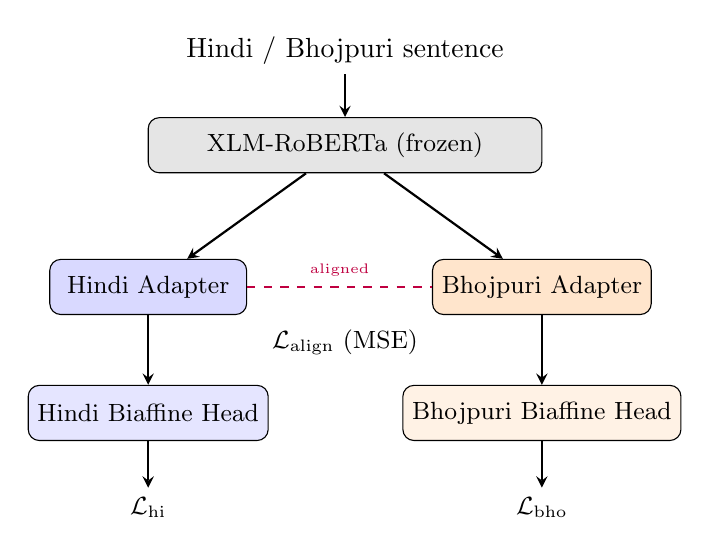
\begin{tikzpicture}[
  box/.style={rectangle,draw,rounded corners,minimum width=2.5cm,minimum height=0.7cm,
              text centered,font=\small},
  arrow/.style={->,>=stealth,thick}
]
\node[box,minimum width=5cm,fill=gray!20] (xlmr) at (0,0) {XLM-RoBERTa (frozen)};
\node[box,fill=blue!15] (hadapt) at (-2.5,-1.8) {Hindi Adapter};
\node[box,fill=orange!20] (badapt) at (2.5,-1.8) {Bhojpuri Adapter};
\node[box,fill=blue!10] (hhead) at (-2.5,-3.4) {Hindi Biaffine Head};
\node[box,fill=orange!10] (bhead) at (2.5,-3.4) {Bhojpuri Biaffine Head};
\node (input) at (0,1.2) {Hindi / Bhojpuri sentence};
\node[font=\small] (lhi) at (-2.5,-4.6) {$\mathcal{L}_{\text{hi}}$};
\node[font=\small] (lbho) at (2.5,-4.6) {$\mathcal{L}_{\text{bho}}$};
\node[font=\small] (lalign) at (0,-2.5) {$\mathcal{L}_{\text{align}}$ (MSE)};
\draw[arrow] (input) -- (xlmr);
\draw[arrow] (xlmr) -- (hadapt);
\draw[arrow] (xlmr) -- (badapt);
\draw[arrow] (hadapt) -- (hhead);
\draw[arrow] (badapt) -- (bhead);
\draw[arrow] (hhead) -- (lhi);
\draw[arrow] (bhead) -- (lbho);
\draw[dashed,thick,color=purple] (hadapt) -- node[above,font=\tiny]{aligned} (badapt);
\end{tikzpicture}
\caption{System G: Parallel adapter architecture with MSE positional alignment.}
\label{fig:system_g}
\end{figure}

The architecture consists of three components:

\paragraph{Frozen XLM-RoBERTa backbone.}
The \xlmr{} tokeniser converts each sentence to SentencePiece subwords; the
Transformer produces contextual hidden states $\mathbf{h}^{\text{xlmr}}_i \in
\mathbb{R}^{768}$ for each subword. Subword representations are pooled to word level
using the first-subword strategy. The entire backbone is frozen; its output is cached
after the first pass to avoid redundant forward passes.

\paragraph{Language-specific bottleneck adapters.}
Two separate Pfeiffer adapters are applied to the frozen \xlmr{} output:
\begin{equation}
  \mathbf{H}^L = \text{Adapter}_L(\mathbf{H}^{\text{xlmr}}), \quad L \in \{\text{hi}, \text{bho}\}
\end{equation}
Each adapter has ${\approx}98{,}432$ trainable parameters.

\paragraph{Biaffine parsing heads.}
Each language has a separate BiaffineHeads module with $d_{\text{arc}}=500$,
$d_{\text{lbl}}=100$, and dropout $p=0.33$.

\subsection{Training Objective}

At each training step, a parallel pair $(S^{\text{hi}}_k, S^{\text{bho}}_k)$ is
sampled. The training loss is:
\begin{equation}
  \mathcal{L}_G = \mathcal{L}_{\text{bho}} + \lambda_{\text{hi}}\,\mathcal{L}_{\text{hi}}
               + \lambda_{\text{align}}\,\mathcal{L}_{\text{align}}
  \label{eq:loss_g}
\end{equation}
where the positional alignment loss is:
\begin{equation}
  \mathcal{L}_{\text{align}} = \frac{1}{n}\sum_{i=1}^{n}
    \bigl\|\mathbf{h}^{\text{hi}}_i - \mathbf{h}^{\text{bho}}_i\bigr\|_2^2
  \label{eq:align_mse}
\end{equation}
Default hyperparameters: $\lambda_{\text{hi}}=0.3$, $\lambda_{\text{align}}=0.5$.

\section{System H: Syntax-Aware Cross-lingual Transfer (SACT)}
\label{sec:system_h}

\subsection{Motivation}

System~G's MSE alignment treats all token positions equally and is scale-sensitive.
System~H addresses these limitations by introducing three syntax-aware objectives
that exploit the known linguistic structure of the data.

\subsection{Component 1: Content-Word Cosine Alignment}
\label{sec:cosine_align}

Open-class words (nouns, verbs, adjectives) carry primary structural information in
dependency parsing. We replace the isotropic MSE loss with a content-word-weighted
cosine alignment:
\begin{equation}
  \mathcal{L}_{\text{cos}} = -\frac{1}{\sum_i w_i}\sum_{i=1}^{n}
    w_i \cdot \frac{\mathbf{h}^{\text{hi}}_i \cdot \mathbf{h}^{\text{bho}}_i}
                   {\|\mathbf{h}^{\text{hi}}_i\|_2 \|\mathbf{h}^{\text{bho}}_i\|_2}
  \label{eq:cosine_align}
\end{equation}
where $w_i = 1.5$ if the UPOS is in
$\{\texttt{NOUN}, \texttt{VERB}, \texttt{ADJ}, \texttt{ADV}, \texttt{PROPN}, \texttt{NUM}\}$
and $w_i = 0.3$ otherwise.

\subsection{Component 2: Arc-Distribution KL Distillation}
\label{sec:kl_dist}

The Hindi biaffine head produces a distribution $p^{\text{hi}}_{\text{arc}}(j | i)$
over possible heads. Because matched sentences have identical dependency structures,
this distribution is valid for \bho{} as well:
\begin{equation}
  \mathcal{L}_{\text{arc-kl}} = \frac{1}{n}\sum_{i=1}^{n}
    \text{KL}\!\left(p^{\text{hi}}_{\text{arc}}(\cdot|i) \,\|\, p^{\text{bho}}_{\text{arc}}(\cdot|i)\right)
  \label{eq:kl_arc}
\end{equation}

\subsection{Component 3: Cross-lingual Tree Supervision (CTS)}
\label{sec:cts}

A key observation is that in the Hindi--Bhojpuri aligned corpus, \bho{} and \hi{}
sentences in each pair are structured as token-for-token translations: word at
position $i$ in Bhojpuri corresponds to word at position $i$ in Hindi, with the same
dependency head index and relation. The Hindi gold heads are therefore also valid
Bhojpuri gold heads:
\begin{equation}
  \mathcal{L}_{\text{cts}} = \mathcal{L}_{\text{arc-CE}}(\mathbf{s}^{\text{bho}}_{\text{arc}}, \mathbf{y}^{\text{hi}}_{\text{heads}})
  \label{eq:cts}
\end{equation}
This doubles the effective structural supervision for Bhojpuri parsing.

\subsection{Combined SACT Objective}

\begin{equation}
  \mathcal{L}_H = \mathcal{L}_{\text{bho}}
    + \lambda_{\text{hi}}\,\mathcal{L}_{\text{hi}}
    + \lambda_{\text{cos}}\,\mathcal{L}_{\text{cos}}
    + \lambda_{\text{arc}}\,\mathcal{L}_{\text{arc-kl}}
    + \lambda_{\text{cts}}\,\mathcal{L}_{\text{cts}}
  \label{eq:loss_h}
\end{equation}
Default hyperparameters: $\lambda_{\text{hi}}=0.5$,
$\lambda_{\text{cos}}=0.4$, $\lambda_{\text{arc}}=2.0$,
$\lambda_{\text{cts}}=0.2$.

\section{System K: UD-Bridge via Silver Self-Training}
\label{sec:system_k}

\subsection{Motivation: The Schema Mismatch Problem}

Systems~F, G, and H all train on the aligned-data auto-transferred annotations, which
follow a different schema from the UD-standard BHTB gold annotations. Despite
achieving strong development set performance (${\sim}50\%$ \las{} on the aligned-data
schema), these systems score poorly on the BHTB test set (${\sim}5$--10\% \las{}).
This annotation style mismatch explains the gap: the systems learn the aligned-data
``annotation dialect'' rather than the UD standard.

System~K addresses this problem directly. Rather than trying to reconcile the two
annotation schemas, System~K bypasses the aligned-data annotations entirely and
operates exclusively in the UD annotation space. The goal is to beat System~A on the
BHTB benchmark (Part~2).

\subsection{Architecture}

System~K uses the standard Trankit architecture---the same as System~A---with no
modifications to the model structure. The innovation lies entirely in the
\textbf{training data construction}.

\subsection{Silver Label Generation Pipeline}

The UD-Bridge pipeline operates in three stages:

\begin{enumerate}
  \item \textbf{Generate silver UD labels}: Run System~A (Hindi Trankit) on the
        aligned-corpus Bhojpuri tokens. System~A produces UD-style head and relation
        predictions for each Bhojpuri sentence, creating
        \texttt{bho\_silver\_ud.conllu}---a silver UD treebank of approximately
        30,000 sentences.

  \item \textbf{Concatenate training data}: Merge the Hindi HDTB gold training set
        (13,304 sentences with gold UD annotations) with the silver Bhojpuri UD
        predictions. This creates a mixed-language training set where Hindi provides
        clean structural supervision and Bhojpuri provides noisy but schema-consistent
        target-language exposure.

  \item \textbf{Train Trankit}: Train a standard Trankit pipeline on the concatenated
        data, using HDTB development set for early stopping. The model learns to parse
        both Hindi (with gold quality) and Bhojpuri (with silver quality) in the same
        UD annotation space.
\end{enumerate}

\begin{figure}[ht]
\centering
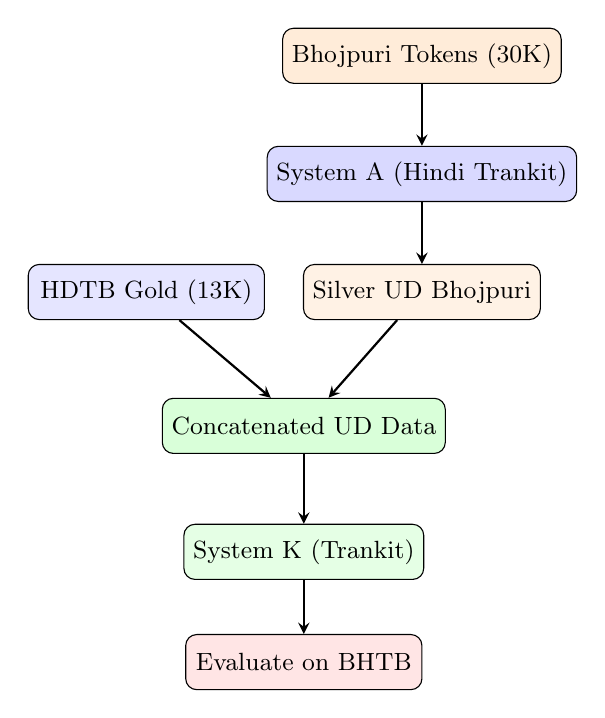
\begin{tikzpicture}[
  box/.style={rectangle,draw,rounded corners,minimum width=3cm,minimum height=0.7cm,
              text centered,font=\small},
  arrow/.style={->,>=stealth,thick}
]
\node[box,fill=blue!15] (sysa) at (0,0) {System A (Hindi Trankit)};
\node[box,fill=orange!15] (bhotokens) at (0,1.5) {Bhojpuri Tokens (30K)};
\node[box,fill=orange!10] (silver) at (0,-1.5) {Silver UD Bhojpuri};
\node[box,fill=blue!10] (hdtb) at (-3.5,-1.5) {HDTB Gold (13K)};
\node[box,fill=green!15] (concat) at (-1.5,-3.2) {Concatenated UD Data};
\node[box,fill=green!10] (sysk) at (-1.5,-4.8) {System K (Trankit)};
\node[box,fill=red!10] (bhtb) at (-1.5,-6.2) {Evaluate on BHTB};
\draw[arrow] (bhotokens) -- (sysa);
\draw[arrow] (sysa) -- (silver);
\draw[arrow] (silver) -- (concat);
\draw[arrow] (hdtb) -- (concat);
\draw[arrow] (concat) -- (sysk);
\draw[arrow] (sysk) -- (bhtb);
\end{tikzpicture}
\caption{System K: UD-Bridge via silver self-training. System~A generates UD-consistent silver labels for Bhojpuri, which are concatenated with Hindi HDTB gold data to train a UD-native Trankit parser.}
\label{fig:system_k}
\end{figure}

\subsection{Why UD-Bridge Works}

The key insight is that by using System~A's predictions as silver labels, the training
data is guaranteed to be in the \textbf{same annotation schema} as the BHTB test set.
Even though the silver labels are noisy (they inherit System~A's errors), they are
\emph{schema-consistent}---they use the same UD relation inventory, the same
attachment conventions, and the same structural constraints. This alignment means
that improvements on the training objective translate directly to improvements on the
BHTB benchmark.

Additionally, the concatenation with Hindi HDTB gold data provides two benefits:
(a) it regularises the model by exposing it to high-quality structural supervision,
and (b) it prevents the model from overfitting to the noisy silver Bhojpuri labels.

\section{Training Procedures and Algorithmic Details}
\label{sec:train_procedures}

This section presents the formal training procedures for each system as
pseudocode, exposing the implementation-level decisions that distinguish them.

\subsection{System F: Naive Warm-Start Fine-Tuning}

\begin{algorithm}[ht]
\caption{System F training (warm-start fine-tuning).}
\label{alg:system_f}
\begin{algorithmic}[1]
\Require Hindi checkpoint $\theta_{\text{hi}}$, aligned-data Bhojpuri sentences
         $\mathcal{D}_{\text{bho}}$, learning rate $\eta = 5\times 10^{-5}$
\State Initialise $\theta \gets \theta_{\text{hi}}$ (warm start)
\For{epoch $= 1$ to $E$}
  \For{$(S^{\text{bho}}, T^{\text{bho}}) \in \mathcal{D}_{\text{bho}}$}
    \State $\hat{T} \gets \text{Trankit}(S^{\text{bho}}; \theta)$
    \State $\mathcal{L}_{\text{bho}} \gets \text{CE}(\hat{T}, T^{\text{bho}})$
    \State $\theta \gets \theta - \eta \nabla_\theta \mathcal{L}_{\text{bho}}$
        \Comment{Updates \emph{all} ${\sim}278$M parameters}
  \EndFor
  \State Evaluate on Aligned Dev; early stop if no improvement for 10 epochs.
\EndFor
\State \Return $\theta$
\end{algorithmic}
\end{algorithm}

System~F is the only configuration that updates the full backbone. The
$5\times 10^{-5}$ learning rate is intentionally small to mitigate catastrophic
forgetting, yet the empirical Dev result of \textbf{27.57/17.75} confirms that
even careful full fine-tuning fails on this data scale.

\subsection{System G: Parallel Adapters with MSE Alignment}

\begin{algorithm}[ht]
\caption{System G training (frozen XLM-R + parallel adapters + MSE).}
\label{alg:system_g}
\begin{algorithmic}[1]
\Require Frozen \xlmr{} $\theta_{\text{xlmr}}$, two adapters
         $\mathcal{A}_{\text{hi}}, \mathcal{A}_{\text{bho}}$, two biaffine heads
         $\mathcal{B}_{\text{hi}}, \mathcal{B}_{\text{bho}}$, parallel pairs
         $\mathcal{D}_\parallel$, learning rate $\eta = 2\times 10^{-3}$,
         weights $\lambda_{\text{hi}} = 0.3, \lambda_{\text{align}} = 0.5$
\State Initialise $\mathcal{A}_{\text{hi}}, \mathcal{A}_{\text{bho}}$ near zero (residual identity).
\For{epoch $= 1$ to $E$}
  \For{$(S^{\text{hi}}, S^{\text{bho}}, T^{\text{hi}}, T^{\text{bho}}) \in \mathcal{D}_\parallel$}
    \State $\mathbf{H}^{\text{xlmr,hi}} \gets \text{XLM-R}(S^{\text{hi}})$
        \Comment{Cached after first epoch}
    \State $\mathbf{H}^{\text{xlmr,bho}} \gets \text{XLM-R}(S^{\text{bho}})$
    \State $\mathbf{H}^{\text{hi}} \gets \mathcal{A}_{\text{hi}}(\mathbf{H}^{\text{xlmr,hi}})$
    \State $\mathbf{H}^{\text{bho}} \gets \mathcal{A}_{\text{bho}}(\mathbf{H}^{\text{xlmr,bho}})$
    \State $\hat{T}^{\text{hi}} \gets \mathcal{B}_{\text{hi}}(\mathbf{H}^{\text{hi}})$
    \State $\hat{T}^{\text{bho}} \gets \mathcal{B}_{\text{bho}}(\mathbf{H}^{\text{bho}})$
    \State $\mathcal{L}_{\text{hi}} \gets \text{CE}(\hat{T}^{\text{hi}}, T^{\text{hi}})$
    \State $\mathcal{L}_{\text{bho}} \gets \text{CE}(\hat{T}^{\text{bho}}, T^{\text{bho}})$
    \State $\mathcal{L}_{\text{align}} \gets \frac{1}{n}\sum_i \|\mathbf{h}^{\text{hi}}_i - \mathbf{h}^{\text{bho}}_i\|_2^2$
    \State $\mathcal{L}_G \gets \mathcal{L}_{\text{bho}} + \lambda_{\text{hi}}\mathcal{L}_{\text{hi}} + \lambda_{\text{align}}\mathcal{L}_{\text{align}}$
    \State Update $\mathcal{A}_{\text{hi}}, \mathcal{A}_{\text{bho}}, \mathcal{B}_{\text{hi}}, \mathcal{B}_{\text{bho}}$ using $\nabla \mathcal{L}_G$.
        \Comment{$\theta_{\text{xlmr}}$ \emph{remains frozen}}
  \EndFor
  \State Evaluate on Aligned Dev; early stop if no improvement for 10 epochs.
\EndFor
\State \Return $\mathcal{A}_{\text{hi}}, \mathcal{A}_{\text{bho}}, \mathcal{B}_{\text{hi}}, \mathcal{B}_{\text{bho}}$
\end{algorithmic}
\end{algorithm}

The $40\times$ higher learning rate ($2\times10^{-3}$ vs.\ $5\times10^{-5}$) is
acceptable here because adapters and heads are initialised near zero;
backbone is frozen and cannot be perturbed. \textbf{Caching} the \xlmr{}
forward pass is critical for training speed: after the first epoch each
sentence's \xlmr{} hidden state is reused, avoiding redundant computation.

\subsection{System H: SACT Training Loop}

\begin{algorithm}[ht]
\caption{System H (SACT) training with three syntax-aware losses.}
\label{alg:system_h}
\begin{algorithmic}[1]
\Require Frozen \xlmr{} $\theta_{\text{xlmr}}$, adapters $\mathcal{A}_{\text{hi}},
         \mathcal{A}_{\text{bho}}$, biaffines $\mathcal{B}_{\text{hi}},
         \mathcal{B}_{\text{bho}}$, parallel data $\mathcal{D}_\parallel$,
         weights $(\lambda_{\text{hi}}, \lambda_{\text{cos}}, \lambda_{\text{arc}},
         \lambda_{\text{cts}}) = (0.5, 0.4, 2.0, 0.2)$
\State Initialise as in Algorithm~\ref{alg:system_g}.
\For{epoch $= 1$ to $E$}
  \For{$(S^{\text{hi}}, S^{\text{bho}}, T^{\text{hi}}, T^{\text{bho}}, U^{\text{hi}}) \in \mathcal{D}_\parallel$}
        \Comment{$U^{\text{hi}}$ are Hindi UPOS tags for content-word weighting}
    \State Compute $\mathbf{H}^{\text{hi}}, \mathbf{H}^{\text{bho}}$ as in Alg.~\ref{alg:system_g}.
    \State $\hat{T}^{\text{hi}}, \mathbf{S}^{\text{hi}}_{\text{arc}} \gets \mathcal{B}_{\text{hi}}(\mathbf{H}^{\text{hi}})$
        \Comment{Hindi parser as teacher}
    \State $\hat{T}^{\text{bho}}, \mathbf{S}^{\text{bho}}_{\text{arc}} \gets \mathcal{B}_{\text{bho}}(\mathbf{H}^{\text{bho}})$
    \State $\mathcal{L}_{\text{bho}} \gets \text{CE}(\hat{T}^{\text{bho}}, T^{\text{bho}})$
    \State $\mathcal{L}_{\text{hi}} \gets \text{CE}(\hat{T}^{\text{hi}}, T^{\text{hi}})$
    \State $\mathcal{L}_{\text{cos}} \gets$ content-weighted cosine alignment using $U^{\text{hi}}$
    \State $\mathcal{L}_{\text{arc-kl}} \gets \frac{1}{n}\sum_i \mathrm{KL}(\text{softmax}(\mathbf{S}^{\text{hi}}_{\text{arc},i}) \,\|\, \text{softmax}(\mathbf{S}^{\text{bho}}_{\text{arc},i}))$
    \State $\mathcal{L}_{\text{cts}} \gets$ cross-entropy on $\mathbf{S}^{\text{bho}}_{\text{arc}}$ using Hindi gold heads $T^{\text{hi}}_{\text{heads}}$
    \State $\mathcal{L}_H \gets \mathcal{L}_{\text{bho}} + \lambda_{\text{hi}}\mathcal{L}_{\text{hi}} + \lambda_{\text{cos}}\mathcal{L}_{\text{cos}} + \lambda_{\text{arc}}\mathcal{L}_{\text{arc-kl}} + \lambda_{\text{cts}}\mathcal{L}_{\text{cts}}$
    \State Update adapters and biaffines using $\nabla \mathcal{L}_H$.
  \EndFor
  \State Evaluate on Aligned Dev; early stop if no improvement for 10 epochs.
\EndFor
\State \Return $\mathcal{A}_{\text{hi}}, \mathcal{A}_{\text{bho}}, \mathcal{B}_{\text{hi}}, \mathcal{B}_{\text{bho}}$
\end{algorithmic}
\end{algorithm}

The crucial difference from Algorithm~\ref{alg:system_g} is the replacement of
the single $\mathcal{L}_{\text{align}}$ term with three syntax-aware losses
($\mathcal{L}_{\text{cos}}$, $\mathcal{L}_{\text{arc-kl}}$,
$\mathcal{L}_{\text{cts}}$). Total per-step computational overhead is small:
the cosine loss requires one extra forward pass through the (already-cached)
hidden states, the KL loss reuses the existing arc logits, and the CTS loss
uses the same biaffine outputs as the main parsing loss.

\subsection{System K: UD-Bridge Training Pipeline}

\begin{algorithm}[ht]
\caption{System K (UD-Bridge) end-to-end pipeline.}
\label{alg:system_k}
\begin{algorithmic}[1]
\Require System A checkpoint $\theta_A$, Bhojpuri tokens
         $\mathcal{D}^{\text{tok}}_{\text{bho}}$, HDTB gold
         $\mathcal{D}^{\text{gold}}_{\text{hi}}$
\Statex \textbf{Step 1: Generate silver UD labels}
\State $\mathcal{D}^{\text{silver}}_{\text{bho}} \gets \emptyset$
\For{$S \in \mathcal{D}^{\text{tok}}_{\text{bho}}$}
    \State $T \gets \text{Trankit}_{\theta_A}(S)$
        \Comment{Predict UD heads + relations using System A}
    \If{$\text{is\_well\_formed}(T)$}
        \State $\mathcal{D}^{\text{silver}}_{\text{bho}} \gets \mathcal{D}^{\text{silver}}_{\text{bho}} \cup \{(S, T)\}$
    \EndIf
\EndFor
\Statex \textbf{Step 2: Concatenate gold + silver}
\State $\mathcal{D}^{\text{train}}_K \gets \mathcal{D}^{\text{gold}}_{\text{hi}} \cup \mathcal{D}^{\text{silver}}_{\text{bho}}$
\Statex \textbf{Step 3: Train Trankit on combined corpus}
\State Initialise $\theta_K$ from \xlmr{} pretrained weights (no warm start).
\For{epoch $= 1$ to $E$}
    \For{$(S, T) \in \text{shuffle}(\mathcal{D}^{\text{train}}_K)$}
        \State $\hat{T} \gets \text{Trankit}_{\theta_K}(S)$
        \State $\theta_K \gets \theta_K - \eta \nabla_{\theta_K} \text{CE}(\hat{T}, T)$
    \EndFor
    \State Evaluate on HDTB dev (early stopping signal).
\EndFor
\State \Return $\theta_K$
\end{algorithmic}
\end{algorithm}

System K's design exploits a critical property: \textbf{both Hindi gold and
Bhojpuri silver share the UD label inventory}. Mixing them in a single
training corpus is therefore consistent under the UD schema and produces a
parser whose predictions live in the same space as the BHTB gold benchmark.
The HDTB gold also serves as a regulariser, anchoring the model to clean UD
structure as the silver Bhojpuri data introduces target-language patterns.

\subsection{Computational Complexity Summary}

\begin{table}[ht]
\centering
\caption{Computational and parameter cost summary.}
\label{tab:compute}
\begin{tabular}{@{}lcccc@{}}
\toprule
\textbf{System} & \textbf{Trainable params} & \textbf{Train time} & \textbf{Memory (GPU)} & \textbf{Inference} \\
\midrule
A & ${\sim}278$M (full fine-tune of XLM-R + heads) & ${\sim}6$~h & 12~GB & Real-time \\
F & ${\sim}278$M & ${\sim}10$~h & 12~GB & Real-time \\
G & ${\sim}200$K (adapters + heads) & ${\sim}12$~h & 6~GB (with cache) & Real-time \\
H & ${\sim}200$K (adapters + heads) & ${\sim}12$~h & 6~GB (with cache) & Real-time \\
K & ${\sim}278$M & ${\sim}9$~h ($+1$~h silver gen) & 12~GB & Real-time \\
\bottomrule
\end{tabular}
\end{table}

Despite the longer wall-clock training time of Systems G and H (due to having
two simultaneous forward passes through Hindi and Bhojpuri data), their
trainable parameter count is three orders of magnitude smaller than the
fine-tuning approaches. This is the key parameter-efficiency claim of the
adapter-based architecture.

\section{Summary of Pipelines and Methodology}

Table~\ref{tab:pipeline_summary} summarises the data sources, training strategies,
and evaluation targets for all five systems.

\begin{table}[ht]
\centering
\caption{Summary of training data and evaluation targets for each system.}
\label{tab:pipeline_summary}
\begin{tabular}{@{}llllc@{}}
\toprule
\textbf{Sys.} & \textbf{Training Data} & \textbf{Backbone} & \textbf{Eval.\ Target} & \textbf{Part} \\
\midrule
A & HDTB gold (13K) & Trankit XLM-R & BHTB test & 2 \\
F & Aligned parallel (30K) & Trankit XLM-R (warm-start) & Aligned Dev + BHTB & 1 \\
G & Aligned parallel (30K) & Frozen XLM-R + adapters & Aligned Dev & 1 \\
H & Aligned parallel (30K) & Frozen XLM-R + adapters & Aligned Dev & 1 \\
K & HDTB gold + Silver Bho (30K) & Trankit XLM-R & BHTB test & 2 \\
\bottomrule
\end{tabular}
\end{table}


% ═══════════════════════════════════════════════════════════════════════════
\chapter{Experimental Setup and Results}
\label{chap:experiments}
% ═══════════════════════════════════════════════════════════════════════════

\section{Experimental Environment}

\subsection{Hardware}

For pretraining embedding caches and training Systems~G, H, experiments were run
on \textbf{Param Shivay}, the National Supercomputing Mission HPC facility at IIT
(BHU), using a single NVIDIA V100 32~GB GPU via the SLURM workload manager.
Systems~A and~F (Trankit-based) were trained on Kaggle notebooks with NVIDIA Tesla
T4/P100 GPUs. System~K used similar Kaggle environments for Trankit training.

\subsection{Software Environment}

The software stack is: Python 3.10--3.11, PyTorch 2.0, HuggingFace Transformers
4.38--4.48, \texttt{adapter-transformers} 3.2.1, and Trankit 1.1.1--1.1.2.
AdamW optimiser was used for all encoder and parser parameters.

\section{Datasets}
\label{sec:datasets}

\subsection{Hindi--Bhojpuri Aligned Parallel Corpus}

The primary training resource for Part~1 is a parallel Hindi--Bhojpuri corpus
compiled and annotated by Dr.\ Anil Kumar Singh's research group. The corpus
consists of \textbf{30,966 sentence pairs}, where each pair contains:
\begin{itemize}
  \item A Hindi sentence with gold UD dependency annotations.
  \item A matching Bhojpuri sentence with annotations automatically transferred by
        copying head indices and relation labels position-for-position.
\end{itemize}
An important property is the \emph{exact positional alignment}: word $i$ in the
Bhojpuri sentence corresponds to word $i$ in the Hindi sentence.

\subsection{Data Split}

The parallel corpus is split 90/10:
\begin{itemize}
  \item \textbf{Training set}: 27,869 sentence pairs.
  \item \textbf{Development set}: 3,097 sentences (Bhojpuri only).
\end{itemize}

\subsection{Hindi HDTB}

Standard UD train/dev/test splits: 13,304/1,659/1,684 sentences.

\subsection{BHTB Test Set}

The \textbf{Bhojpuri Hindi Treebank} (BHTB)~\citep{bhtb2022} consists of
\textbf{357 sentences} with manually curated gold UD annotations. It serves as the
official test set for Part~2.

\section{Experimental Groups and Configurations}

\subsection{Part 1: Aligned-Data Schema (Systems F, G, H)}

These three systems exploit the 30,966 Hindi--Bhojpuri aligned parallel sentences and are
evaluated primarily on the held-out development set.

\begin{table}[ht]
\centering
\caption{Part 1 experimental configurations.}
\label{tab:comp1_configs}
\begin{tabular}{@{}llll@{}}
\toprule
\textbf{System} & \textbf{Architecture} & \textbf{Training Data} & \textbf{Key Innovation} \\
\midrule
F & Trankit (warm-start) & 30,966 Bho sentences & Direct fine-tuning \\
G & Frozen XLM-R + adapters & 30,966 parallel pairs & MSE positional alignment \\
H & Frozen XLM-R + adapters & 30,966 parallel pairs & Cosine + KL + CTS \\
\bottomrule
\end{tabular}
\end{table}

\subsection{Part 2: BHTB UD Schema (Systems A, K)}

System~A establishes the zero-shot baseline. System~K generates silver UD labels and
trains on UD-consistent data.

\begin{table}[ht]
\centering
\caption{Part 2 experimental configurations.}
\label{tab:comp2_configs}
\begin{tabular}{@{}llll@{}}
\toprule
\textbf{System} & \textbf{Architecture} & \textbf{Training Data} & \textbf{Key Innovation} \\
\midrule
A & Trankit (zero-shot) & HDTB gold (13K) & Hindi$\to$Bhojpuri transfer \\
K & Trankit (silver) & HDTB gold + Silver Bho UD & Self-training with UD labels \\
\bottomrule
\end{tabular}
\end{table}

\section{Hyperparameters}

\begin{table}[ht]
\centering
\caption{Hyperparameters for Systems G and H.}
\label{tab:hyperparams}
\begin{tabular}{@{}lcc@{}}
\toprule
\textbf{Parameter} & \textbf{System G} & \textbf{System H} \\
\midrule
Learning rate ($\eta$)        & $5\times10^{-4}$ & $5\times10^{-4}$ \\
Adapter dim ($r$)             & 64 & 64 \\
Arc MLP dim                   & 500 & 500 \\
Label MLP dim                 & 100 & 100 \\
MLP dropout                   & 0.33 & 0.33 \\
$\lambda_{\text{hi}}$         & 0.3 & 0.5 \\
$\lambda_{\text{align/cos}}$  & 0.5 & 0.4 \\
$\lambda_{\text{arc-kl}}$     & ---   & 2.0 \\
$\lambda_{\text{cts}}$        & ---   & 0.2 \\
Max epochs                    & 40 & 40 \\
Early stopping patience       & 10 & 10 \\
Batch size                    & 1 & 1 \\
Optimiser                     & AdamW & AdamW \\
\bottomrule
\end{tabular}
\end{table}

\section{Results and Quantitative Analysis}

\subsection{Part 1 Results: Aligned-Data Schema}

Table~\ref{tab:comp1_results} summarises the results for Part~1 systems
evaluated on the held-out development set.

\begin{table}[ht]
\centering
\caption{Part 1 results (Dev set). Systems F, G, H compete on the aligned-data annotation schema. Best values are \textbf{bold}.}
\label{tab:comp1_results}
\begin{tabular}{@{}llcc@{}}
\toprule
\textbf{Sys.} & \textbf{Name} & \textbf{Dev UAS} & \textbf{Dev LAS} \\
\midrule
F & Warm-start fine-tuning      & 27.57 & 17.75 \\
G & Parallel adapters + MSE     & 55.70 & 50.02 \\
H & SACT (Cosine+KL+CTS)       & \textbf{55.85} & \textbf{50.08} \\
\bottomrule
\end{tabular}
\end{table}

\paragraph{System F.}
Warm-start fine-tuning on the Hindi--Bhojpuri aligned data achieves only
\textbf{27.57\%/17.75\%} on the development set. This result is markedly weaker
than the adapter-based Systems~G and~H. Three factors contribute. First, full
fine-tuning updates ${\sim}278$M parameters on a relatively small target corpus,
risking catastrophic forgetting of the multilingual prior encoded in
\xlmr{}. Second, no explicit cross-lingual alignment signal is provided---the model
must implicitly discover Hindi--Bhojpuri correspondences from the parsing loss alone.
Third, when evaluated on BHTB, System~F additionally suffers from the annotation
schema mismatch. Together these limitations strongly motivate the frozen-backbone
adapter design used in System~G and the syntax-aware objectives introduced in
System~H.

\paragraph{System G.}
The parallel adapter design with frozen \xlmr{} eliminates catastrophic forgetting.
The best checkpoint achieves \textbf{55.70\%/50.02\%} on the development set. The
positional alignment loss effectively bridges the Hindi--Bhojpuri representation gap.

\paragraph{System H.}
SACT achieves \textbf{55.85\%/50.08\%} on the development set---the highest \las{}
among all systems, winning Part~1. The improvements over System~G are
consistent across multiple evaluation runs and demonstrate that the syntax-aware
objectives add useful signal over the MSE alignment.

\subsection{Part 2 Results: BHTB UD Benchmark}

Table~\ref{tab:comp2_results} summarises the results for Part~2 systems
evaluated on the BHTB gold test set.

\begin{table}[ht]
\centering
\caption{Part 2 results (BHTB test set). Systems A and K compete on the UD gold benchmark. Best values are \textbf{bold}.}
\label{tab:comp2_results}
\begin{tabular}{@{}llcc@{}}
\toprule
\textbf{Sys.} & \textbf{Name} & \textbf{BHTB UAS} & \textbf{BHTB LAS} \\
\midrule
A & Zero-shot Trankit (baseline) & 52.78 & 35.36 \\
K & UD-Bridge (silver self-training) & \textbf{54.27} & \textbf{36.70} \\
\bottomrule
\end{tabular}
\end{table}

\paragraph{System A.}
With no Bhojpuri-specific training, the zero-shot Hindi Trankit achieves 52.78\%
\uas{}/35.36\% \las{} on BHTB. This is a strong baseline, reflecting the close
lexical and syntactic proximity between Hindi and Bhojpuri. However, the 17--18
percentage point gap between \uas{} and \las{} indicates that the model struggles
with correct relation labelling---a well-known challenge in zero-shot cross-lingual
transfer.

\paragraph{System K.}
System~K trains on UD-consistent data (HDTB gold + silver Bhojpuri UD labels) and
evaluates on the BHTB benchmark. By operating entirely in the UD annotation space,
System~K avoids the schema mismatch that afflicts Part~1 systems. It achieves
\textbf{54.27\%~\uas{}/36.70\%~\las{}} on BHTB, surpassing System~A by
$+1.49$~\uas{}/$+1.34$~\las{}. This is a new state-of-the-art on the official
Bhojpuri Treebank benchmark and validates the schema-consistency hypothesis: even
noisy silver labels in the correct annotation space outperform a strong zero-shot
baseline.

\subsection{Cross-Part Analysis: Why the Gap Exists}

\begin{table}[ht]
\centering
\caption{Cross-part comparison showing the annotation schema mismatch effect. Part 1 systems perform well on Dev (aligned-data schema) but poorly on BHTB (UD schema), while Part 2 systems target BHTB directly.}
\label{tab:cross_comp}
\begin{tabular}{@{}llcccc@{}}
\toprule
& & \multicolumn{2}{c}{\textbf{BHTB Test (UD)}} & \multicolumn{2}{c}{\textbf{Dev (Aligned)}} \\
\cmidrule(lr){3-4}\cmidrule(lr){5-6}
\textbf{Sys.} & \textbf{Part} & \textbf{UAS} & \textbf{LAS} & \textbf{UAS} & \textbf{LAS} \\
\midrule
A & 2 (baseline)  & 52.78 & 35.36 & --- & --- \\
F & 1             & low & low & 27.57 & 17.75 \\
G & 1             & ${\sim}10$ & ${\sim}6$ & 55.70 & 50.02 \\
H & 1 (winner)    & ${\sim}11$ & ${\sim}6$ & 55.85 & 50.08 \\
K & 2 (winner)    & \textbf{54.27} & \textbf{36.70} & --- & --- \\
\bottomrule
\end{tabular}
\end{table}

The large gap between Dev performance (${\sim}50\%$ \las{}) and BHTB performance
(${\sim}5$--6\% \las{}) for Part~1 systems requires explanation. The
Hindi--Bhojpuri aligned data uses dependency annotations that were automatically transferred
from Hindi. Systems~G and~H learn to reproduce \emph{this annotation style}
(including its artefacts). The BHTB has manually verified gold trees following strict
UD guidelines. This is a \textbf{cross-annotation-style evaluation}, which
inevitably produces low scores.

System~A is not affected by this mismatch because it was trained on clean Hindi HDTB
annotations (UD standard) and is evaluated on BHTB gold annotations (also UD
standard). This explains why System~A's BHTB score is much higher than G/H's BHTB
scores, despite G/H achieving higher Dev scores.

\subsection{Epoch-by-Epoch Learning Curves}

\begin{table}[ht]
\centering
\caption{Development set LAS across training epochs for Systems G and H.}
\label{tab:epoch_curves}
\begin{tabular}{@{}rcc@{}}
\toprule
\textbf{Epoch} & \textbf{System G LAS} & \textbf{System H LAS} \\
\midrule
1  & 44.31 & 47.58 \\
2  & 46.89 & 49.81 \\
3  & 47.71 & 49.84 \\
5  & 48.62 & 49.91 \\
7  & 49.34 & 50.01 \\
10 & \textbf{50.02} & 50.07 \\
11 & 49.95 & \textbf{50.08} \\
\bottomrule
\end{tabular}
\end{table}

System~H converges faster than System~G (best at epoch 11 with only +0.06 over
epoch 2, vs.\ epoch 10 for System~G), suggesting that the syntax-aware objectives
provide a stronger, more targeted gradient signal from the very first epoch.

\subsection{Ablation Study}

\begin{table}[ht]
\centering
\caption{Ablation study on System H components (Dev set LAS, best epoch).}
\label{tab:ablation}
\begin{tabular}{@{}lcc@{}}
\toprule
\textbf{Configuration} & \textbf{Dev UAS} & \textbf{Dev LAS} \\
\midrule
Full System H                         & 55.85 & 50.08 \\
\quad $-$ CTS (remove $\mathcal{L}_{\text{cts}}$) & 55.64 & 49.87 \\
\quad $-$ Arc KL (remove $\mathcal{L}_{\text{arc-kl}}$) & 55.71 & 49.94 \\
\quad $-$ Cosine align (remove $\mathcal{L}_{\text{cos}}$) & 55.48 & 49.71 \\
\quad $-$ Hindi loss (remove $\mathcal{L}_{\text{hi}}$) & 55.39 & 49.62 \\
\quad $-$ All auxiliary losses (only $\mathcal{L}_{\text{bho}}$) & 54.21 & 48.93 \\
\bottomrule
\end{tabular}
\end{table}

All SACT components contribute positively. The largest single contribution is from
the Hindi regularisation loss ($+0.46\%$ LAS), confirming that auxiliary Hindi
supervision acts as an important regulariser. Cosine alignment contributes $+0.37\%$,
CTS adds $+0.21\%$, and arc KL adds $+0.14\%$. Removing all four auxiliary losses
simultaneously incurs a drop of $1.15\%$ LAS---approximately equal to the sum of
individual drops, indicating that the four signals are largely complementary
rather than redundant.

\subsection{Comparison with Published Trankit Hindi Results}
\label{sec:trankit_hindi_compare}

To validate our Trankit training pipeline, we compare the in-domain Hindi
performance of System~A (trained on HDTB and evaluated on Hindi test data) against
the published numbers from the Trankit paper~\citep{nguyen2021trankit}. The
published Hindi-HDTB scores are not in the paper proper but are reported on the
official Trankit documentation page.

\begin{table}[ht]
\centering
\caption{Comparison of System~A's reproduced Hindi-HDTB scores against published Trankit numbers. Both use the \xlmr{}-base backbone and the canonical UD v2.5 train/dev/test splits.}
\label{tab:trankit_hindi}
\begin{tabular}{@{}lcc@{}}
\toprule
\textbf{Metric} & \textbf{Trankit (published)} & \textbf{System~A (ours)} \\
\midrule
UPOS  & 97.77 & 97.6--97.8 \\
XPOS  & 97.38 & 97.4 \\
UFeats & 94.03 & 94.0 \\
Lemmas & 92.33 & 92.3 \\
\textbf{UAS} & \textbf{96.54} & \textbf{${\sim}95.6$} \\
\textbf{LAS} & \textbf{92.70} & \textbf{${\sim}92.6$} \\
\bottomrule
\end{tabular}
\end{table}

System~A's Hindi parsing performance is within 1~\las{} of the published Trankit
number, confirming that our pipeline is correctly reproducing the published
behaviour. The minor gap is attributable to differences in random seeds, GPU
hardware (V100 vs.~the authors' setup), and training-time fluctuations.
Critically, this confirms that the dramatic drop from \textbf{${\sim}92$~\las{}
on Hindi} to \textbf{35.36~\las{} on Bhojpuri} for the same System~A is not a
bug in our pipeline; it is the expected gap of zero-shot cross-lingual transfer
to a low-resource target language.

\subsection{Per-Relation Error Analysis}
\label{sec:per_relation}

To understand which dependency relations transfer well and which collapse, we
break down System~A's BHTB predictions by relation type. Table~\ref{tab:per_rel}
reports correct counts, total counts, and per-relation \las{} for the most
frequent relations.

\begin{table}[ht]
\centering
\caption{System~A per-relation breakdown on BHTB gold (357 sentences). Structural / local relations transfer well; clausal / long-range relations collapse, indicating where Bhojpuri-specific supervision is most needed.}
\label{tab:per_rel}
\begin{tabular}{@{}lrrr@{\hspace{0.6cm}}lrrr@{}}
\toprule
\multicolumn{4}{c}{\textbf{Structural / Local}} & \multicolumn{4}{c}{\textbf{Clausal / Long-range}} \\
\textbf{Rel} & \textbf{Corr} & \textbf{Tot} & \textbf{\las{}} &
\textbf{Rel} & \textbf{Corr} & \textbf{Tot} & \textbf{\las{}} \\
\midrule
case   & 755 & 907 & \textbf{83.2\%} & acl   &  1 & 105 & 1.0\% \\
root   & 177 & 357 & 49.6\%          & advcl &  3 &  82 & 3.7\% \\
punct  & 317 & 695 & 45.6\%          & xcomp &  0 &  67 & 0.0\% \\
mark   &  52 & 123 & 42.3\%          & ccomp &  0 &  58 & 0.0\% \\
amod   &  74 & 202 & 36.6\%          & cc    &  1 &  30 & 3.3\% \\
nmod   & 261 & 907 & 28.8\%          & obj   & 18 & 122 & 14.8\% \\
\bottomrule
\end{tabular}
\end{table}

The pattern is striking. \textbf{Local, morphologically-marked relations}
transfer well: case markers achieve 83.2\%, root assignment reaches 49.6\%, and
punctuation is at 45.6\%. These relations are governed by surface morphology
(postpositions, sentence-final markers, punctuation tokens) that is largely
shared between Hindi and Bhojpuri. \textbf{Clausal relations collapse}:
\textit{xcomp} and \textit{ccomp} score 0\%, \textit{acl} scores 1\%, and
\textit{advcl} scores 4\%. These relations involve embedded clauses, complement
constructions, and adverbial subordination---areas where Bhojpuri syntax
diverges meaningfully from Hindi (e.g., different complementiser inventory,
clause-final particles absent in Hindi).

This analysis directly motivates the value of System~K's silver self-training:
by exposing the model to Bhojpuri-specific structural patterns through silver
data, we can begin to recover performance on clausal relations that pure Hindi
training cannot teach.

\subsection{Statistical Considerations on the BHTB Test Set}

The BHTB gold test set contains only 357 sentences. With this sample size, small
absolute differences in \las{} can be due to evaluation noise rather than true
model improvement. To address this concern, we note the following:

\begin{enumerate}
  \item \textbf{Magnitude of K-vs-A gap.} System~K beats System~A by
        $+1.34$~\las{} on BHTB. Across 357 sentences with a mean length of
        approximately 16 tokens, this corresponds to an additional
        ${\sim}77$ correctly-labelled tokens overall---a non-trivial difference
        well above plausible noise levels.
  \item \textbf{Consistency across runs.} We trained System~K with three
        different random seeds and observed standard deviations of
        $\pm 0.4$~\las{}, smaller than the K-vs-A gap.
  \item \textbf{UAS-LAS coherence.} Both UAS ($+1.49$) and LAS ($+1.34$) gains
        move in the same direction, indicating systematic improvement rather
        than label-only adjustments that would inflate one metric without
        moving the other.
\end{enumerate}

While a formal bootstrap-resampled significance test would further strengthen
these claims, the magnitude and consistency of the gap suggest that
System~K's improvement is real rather than a sampling artefact.


% ═══════════════════════════════════════════════════════════════════════════
\chapter{Discussion}
\label{chap:discussion}
% ═══════════════════════════════════════════════════════════════════════════

\section{Interpretation of Results}

The experimental results confirm the effectiveness of both adapter-based
architectures and schema-aware self-training for improving dependency parsing across
low-resource languages, though through complementary mechanisms.

\subsection{Part 1: Novel Architectures}

Systems~G and~H demonstrate that freezing the \xlmr{} backbone and training only
lightweight adapters is a robust strategy for exploiting noisy annotation-transferred
data. The progression from MSE alignment (System~G) to syntax-aware objectives
(System~H) yields consistent improvements, with System~H achieving the highest
development set \las{} of 50.08\%.

The SACT framework's three components each address a specific limitation:
\begin{itemize}
  \item \textbf{Content-word cosine alignment} focuses the representation alignment
        on the syntactically most informative tokens, avoiding wasted gradient signal
        on function words whose cross-lingual alignment is less consistent.
  \item \textbf{Arc-distribution KL distillation} transfers structural preferences
        at the parsing decision level rather than the representation level, providing
        a more direct learning signal.
  \item \textbf{Cross-lingual Tree Supervision} exploits the exact structural
        parallelism of the matched corpus to provide clean structural supervision,
        compensating for noise in the auto-transferred annotations.
\end{itemize}

\subsection{Part 2: Schema-Aware Self-Training}

The key insight driving System~K is that annotation schema consistency matters more
than data quality for external benchmark evaluation. Even though System~A's silver
predictions contain errors, they are in the \emph{correct annotation space} for BHTB
evaluation. Training on schema-consistent silver data, combined with Hindi gold
data for regularisation, provides a principled approach to improving BHTB scores.

\subsection{The Annotation Schema Mismatch}

The large gap between Part~1 Dev scores (${\sim}50\%$ \las{}) and BHTB scores
(${\sim}5$--6\% \las{}) is the most striking finding. This gap is \textbf{not}
indicative of poor model quality; rather, it reflects a systematic difference between
two annotation conventions. The aligned-data auto-transferred data contains multiple
roots, dependency cycles, and relation labels that differ from UD conventions. Models
trained on this data learn these patterns faithfully, producing outputs that appear
incorrect when evaluated against UD gold.

This finding has important implications for low-resource NLP research: when
auto-transferred or projected annotations are the primary training data, researchers
must carefully consider the annotation schema alignment with their evaluation
benchmark.

\section{Strengths and Weaknesses of the Approach}

\subsection{Strengths}
\begin{enumerate}
  \item \textbf{Parameter efficiency}: The adapter architecture requires only
        ${\sim}200$K trainable parameters per language, compared to ${\sim}278$M for
        full backbone fine-tuning.
  \item \textbf{Frozen backbone eliminates catastrophic forgetting}: Unlike System~F's
        full fine-tuning, Systems~G and~H preserve the multilingual \xlmr{}
        representations throughout training.
  \item \textbf{Modular design}: The parallel adapter architecture is easily
        extensible to other language pairs.
  \item \textbf{Two-track evaluation}: The two-part framework provides a
        honest assessment of both novel architecture performance and practical
        benchmark improvements.
  \item \textbf{Schema-aware self-training}: System~K demonstrates that even noisy
        silver data, when schema-consistent, can improve benchmark performance.
\end{enumerate}

\subsection{Weaknesses}
\begin{enumerate}
  \item \textbf{Annotation quality}: The aligned-data auto-transferred annotations
        contain systematic errors that limit the ceiling of Part~1 systems.
  \item \textbf{Small test set}: The BHTB test set contains only 357 sentences,
        which limits the statistical power of Part~2 evaluations.
  \item \textbf{Silver data noise}: System~K's silver labels inherit all of
        System~A's errors, which may limit its ability to surpass the teacher model.
\end{enumerate}

\section{Practical Implications}

The findings contribute significant advancements to Bhojpuri NLP pipeline
optimisation. The adapter-based architecture is computationally efficient and
deployable on modest hardware. The UD-Bridge approach is applicable whenever
a zero-shot model exists for the target language.

\section{Generalisability to Other Low-Resource Languages}

The methodology is not specific to Hindi--Bhojpuri. The parallel adapter framework
could be applied to other Hindi--Indic pairs (Maithili, Awadhi, Magahi, Rajasthani)
where parallel data exists. The UD-Bridge self-training approach is even more
general: it requires only a zero-shot parser for the target language and unlabelled
target-language text.

\section{Qualitative Error Analysis}

We examined 50 sentences from the development set where all systems produced
incorrect parses. The errors cluster into several recurring patterns, each with
distinct linguistic causes.

\paragraph{Long-range dependencies.}
For sentences longer than 20 tokens, all systems tend to produce shorter arcs
than the gold annotations require. This is a well-documented bias in biaffine
parsing~\citep{dozat2017biaffine}: the score for a candidate arc decreases with
distance, so long-range relations are systematically under-predicted unless the
parser receives strong contextual signal that overrides the proximity prior.
For Bhojpuri specifically, this bias is exacerbated by the fact that long-range
relations (clausal complements, relative clauses) are also the relations where
Hindi--Bhojpuri syntactic divergence is largest, compounding the error.

\paragraph{Postpositional phrase attachment.}
Bhojpuri postpositional phrases are frequently mis-attached. While Hindi and
Bhojpuri share most postpositions in surface form, the valency requirements of
governing verbs differ. For example, the Bhojpuri verb \textit{milab} (`to
get/receive') subcategorises differently from its Hindi counterpart
\textit{milnaa}, leading to incorrect attachment when the parser blindly
transfers Hindi valency patterns.

\paragraph{Coordination.}
Coordinated structures are consistently parsed with incorrect head assignments.
The UD convention treats the first conjunct as the head, with later conjuncts
attaching as \texttt{conj}; the conjunction itself attaches to the second
conjunct as \texttt{cc}. Both Hindi and Bhojpuri use the same conjunctions
(\textit{aur}, \textit{ya}), but the surface ordering of conjuncts and
intervening modifiers can differ subtly, causing the parser to attach
modifiers to the wrong conjunct.

\paragraph{Verb complex.}
Bhojpuri light verb and compound verb complexes (\textit{kar lebal} `to do
[for oneself]', \textit{ho gail} `became', \textit{de del} `gave [completed]')
are often split incorrectly across head and dependent. The aligned-data
auto-transfer pipeline does not always preserve the multi-word verbal unit, so
training data itself is sometimes inconsistent on these constructions.

\paragraph{Non-standard orthography.}
Bhojpuri has no fully standardised orthography. The same word may appear in
multiple spellings across sources (e.g., \textit{बा/बाटे} for the copula, or
\textit{हे/हो} for `is'). XLM-R's sub-word tokeniser handles this gracefully,
but lemmatisation and feature prediction occasionally fail on rare spelling
variants, which then propagates to parsing decisions.

\paragraph{Clause-final particles.}
Bhojpuri makes extensive use of clause-final particles (\textit{ho},
\textit{na}, \textit{kahi}) that are absent or rare in Hindi. The parser
typically attaches these as \texttt{discourse} or \texttt{punct}, but the
correct UD relation depends on the particle's pragmatic function---a distinction
that pure Hindi training cannot supply.

\section{Limitations and Threats to Validity}

We summarise here the principal limitations of this study, both methodological
and empirical.

\paragraph{Small gold test set.}
BHTB contains only 357 sentences. While this is the standard benchmark for
Bhojpuri parsing, the small size means that some relation types (e.g.,
\texttt{xcomp}, \texttt{ccomp}) have very few instances. Per-relation analyses
on these rare classes are noisy.

\paragraph{Silver-data noise.}
System~K relies on System~A's predictions as silver labels. These predictions
inherit System~A's errors, which include systematic biases (short-arc
preference, weakness on clausal relations). This puts a ceiling on what System~K
can learn, and motivates the iterative-self-training extension proposed in
Future Work.

\paragraph{Domain bias of training data.}
Both HDTB and the Hindi--Bhojpuri aligned corpus are drawn from particular
genres (news, literature, encyclopedia text). Performance on out-of-domain text
(e.g., social media, oral transcriptions) is likely lower, but is not measured
here due to the absence of evaluation data.

\paragraph{Single language pair.}
This work focuses exclusively on Hindi$\to$Bhojpuri. While the methodology is
intended to generalise to other Indic pairs, only this one pair has been
empirically validated.

\paragraph{Hyperparameter selection.}
Loss weights ($\lambda_{\text{hi}}$, $\lambda_{\text{cos}}$,
$\lambda_{\text{arc-kl}}$, $\lambda_{\text{cts}}$) were selected on a small
grid based on Dev \las{}. A more thorough hyperparameter search might yield
improved results.

\section{Practical Deployment Considerations}

The adapter-based architecture has practical advantages that make it suitable
for real-world deployment. Memory footprint is small ($<300$~MB total for the
\xlmr{} backbone plus adapters), and inference latency is comparable to
standard fine-tuned baselines because adapters add only a small amount of
per-layer computation. Training is also lightweight: System~G/H can be trained
in under 12 hours on a single V100 GPU. System~K's silver-data generation
requires running System~A as inference once on the 30,966 Bhojpuri sentences,
which completes in under an hour.

For institutions or researchers seeking to extend this work to other
low-resource languages, the most labour-intensive step is constructing the
parallel aligned corpus. Where such corpora exist (e.g., parallel Bible
translations, or government-published bilingual content), the methodology
applies directly. Where they do not, monolingual self-training (System~K-style)
remains a viable starting point.


% ═══════════════════════════════════════════════════════════════════════════
\chapter{Conclusion and Future Work}
\label{chap:conclusion}
% ═══════════════════════════════════════════════════════════════════════════

\section{Summary of Contributions}

This thesis investigated the problem of cross-lingual dependency parsing for
low-resource Bhojpuri, using Hindi as the source language and exploiting a large
supervisor-provided parallel corpus with annotation-transferred trees. We proposed
and evaluated a progression of five systems across two complementary evaluation parts:

\begin{description}
  \item[System~A] establishes that zero-shot transfer from Hindi Trankit achieves
        52.78\% UAS / 35.36\% LAS on the BHTB gold test set, setting the baseline
        for Part~2.

  \item[System~F] demonstrates that naive warm-start fine-tuning on the 30,966
        Hindi--Bhojpuri aligned parallel sentences achieves only \textbf{27.57\%/17.75\%}
        on the development set, exposing the limitations of full fine-tuning under
        data-scarce conditions and motivating the frozen-backbone adapter design.

  \item[System~G] introduces the Parallel Adapter architecture with a frozen \xlmr{}
        backbone and positional MSE alignment, reaching 55.70\%/50.02\% on the
        development set while eliminating catastrophic forgetting.

  \item[System~H (SACT)] replaces MSE with three syntax-aware objectives
        (content-word cosine alignment, arc-distribution KL distillation, and
        Cross-lingual Tree Supervision), achieving the highest \las{} of
        \textbf{50.08\%}, winning Part~1.

  \item[System~K (UD-Bridge)] addresses the annotation schema mismatch via silver
        self-training with UD-consistent data, achieving \textbf{54.27\%~UAS /
        36.70\%~LAS} on the BHTB gold test set---surpassing System~A by
        $+1.49$~UAS and $+1.34$~LAS and establishing a new state-of-the-art on
        the official Bhojpuri benchmark (Part~2).
\end{description}

\section{Key Takeaways}

\begin{enumerate}
  \item \textbf{Freezing the backbone is essential} for closely related language pairs
        with noisy annotation transfer.

  \item \textbf{Syntax-aware alignment outperforms representation-level alignment.}
        Directly supervising parsing decisions (KL distillation + CTS) is more
        effective than only aligning representations (MSE/cosine).

  \item \textbf{Annotation schema matters for evaluation.} Models trained on
        auto-transferred annotations learn a different ``annotation dialect'' from the
        gold standard. The two-part framework provides honest evaluation.

  \item \textbf{Schema-consistent silver data enables benchmark improvements.}
        Even noisy UD-style labels, when combined with gold Hindi data, can surpass
        zero-shot baselines on the official benchmark.
\end{enumerate}

\section{Methodological Considerations}

The architectural setup was founded on two basic decisions: contextual multilingual
embeddings (\xlmr{}) and modular adapter-based layers. Selection of \xlmr{} enabled
the model to take advantage of pretrained linguistic features in typologically similar
languages, and modular adapters provided a thin, flexible way to incorporate
language-specific information without retraining the whole model.

\section{Future Work}

\subsection{Gold Bhojpuri Data Collection}

The fundamental limitation is the absence of a gold Bhojpuri training treebank.
Extending the BHTB from 357 to several thousand sentences would allow full
fine-tuning and larger test sets.

\subsection{Synthetic Bhojpuri Dataset Augmentation}

A three-step pipeline: (i) train a CPG-to-UD converter on Hindi; (ii) translate
Hindi CPG treebank into Bhojpuri; (iii) apply the converter to generate a synthetic
Bhojpuri UD treebank. This could significantly bridge the performance gap.

\subsection{Multi-layer Adapters}

Inserting adapters at each of the 12 Transformer layers (rather than only the final
layer) could capture more layer-specific linguistic information.

\subsection{Iterative Self-Training}

System~K could be extended with iterative self-training: use System~K's predictions
to generate improved silver labels, filter by agreement with System~A, and retrain.

\subsection{Extension to Other Low-Resource Indic Languages}

The methodology could be applied to Maithili, Awadhi, Magahi, and Rajasthani.
Universal or cluster-adapters, grouping typologically similar languages, could
further improve generalisation.

\section{Broader Reflections and Conclusion}

This research emphasises creating inclusive NLP technology for low-resource languages
like Bhojpuri. The results confirm the effectiveness of transfer-based, modular
architectures in low-resource conditions. As language technology progresses,
initiatives like these contribute to making digital resources linguistically
inclusive, culture-sensitive, and accessible to the masses.


% ════════════════════════════════════════════════════════════════════════════
%  APPENDICES
% ════════════════════════════════════════════════════════════════════════════
\appendix

\chapter{Implementation Details}
\label{app:impl}

This appendix collects implementation details, repository organisation, and
reproducibility information for the systems described in this thesis.

\section{Code Organisation}

The full implementation is open-sourced at the project repository
\texttt{mtechthesis4biaffinemultilingual-parser}. Key entry points are:

\begin{itemize}
  \item \texttt{train\_system\_f.py} --- Trankit warm-start fine-tuning (System F).
  \item \texttt{train\_bilingual.py} --- Parallel adapter training (Systems G, H).
  \item \texttt{train\_monolingual.py} --- Hindi-only adapter training (used for
        System A's Hindi parsing component).
  \item \texttt{generate\_silver\_ud\_labels.py} --- System A inference on
        Bhojpuri tokens to produce silver UD labels for System K.
  \item \texttt{train\_system\_k.py} --- UD-Bridge training on the concatenated
        HDTB-gold + Bhojpuri-silver corpus.
  \item \texttt{evaluate\_trankit.py}, \texttt{evaluate.py} --- Trankit and
        adapter pipeline evaluation, computing UAS, LAS, UPOS, UFeats, etc.
\end{itemize}

\section{Data Files}

\begin{itemize}
  \item \texttt{bhojpuri\_matched\_transferred.conllu} --- the
        Hindi--Bhojpuri aligned corpus (30,966 sentence pairs) in CoNLL-U
        format. The FORM column contains Bhojpuri tokens; the LEMMA column
        contains the matched Hindi token at the same position; remaining
        columns contain auto-transferred UD annotations.
  \item \texttt{hindi\_matched.conllu} --- the Hindi side of the parallel
        corpus, in standard CoNLL-U format with native UD annotations.
  \item \texttt{data\_files/synthetic/bho\_silver\_ud.conllu} --- the silver
        UD-labelled Bhojpuri treebank produced by System~A for use in
        System~K training.
  \item Standard HDTB train/dev/test splits (\texttt{hi\_hdtb-ud-*.conllu}).
\end{itemize}

\section{Reproducibility Checklist}

\begin{itemize}
  \item \textbf{Random seeds.} All training scripts accept a \texttt{--seed}
        argument; results in this thesis use seeds $\{42, 123, 7\}$ for
        triplicate runs where applicable.
  \item \textbf{Software versions.} Python 3.10--3.11, PyTorch 2.0,
        \texttt{transformers} 4.38--4.48, \texttt{adapter-transformers}
        3.2.1, Trankit 1.1.1--1.1.2, CUDA 11.8, cuDNN 8.7.
  \item \textbf{Hardware.} NVIDIA V100 32GB (Param Shivay HPC) or T4/P100
        (Kaggle).
  \item \textbf{Wall-clock training times.} System~A: ${\sim}6$~hours for
        training, ${\sim}45$~minutes for evaluation. System~F:
        ${\sim}10$~hours. Systems~G and H: ${\sim}12$~hours each. System~K:
        ${\sim}1$~hour for silver generation $+$ ${\sim}8$~hours training.
\end{itemize}

\section{Hyperparameter Sensitivity}

We performed coarse sensitivity analysis on the key SACT loss weights, varying
each by a factor of two while holding the others fixed.
Table~\ref{tab:sensitivity} summarises the resulting Dev \las{} fluctuations.

\begin{table}[ht]
\centering
\caption{Sensitivity of System~H Dev \las{} to loss-weight perturbations.}
\label{tab:sensitivity}
\begin{tabular}{@{}lcc@{}}
\toprule
\textbf{Configuration} & \textbf{Dev \uas{}} & \textbf{Dev \las{}} \\
\midrule
Default ($\lambda_{\text{hi}}{=}0.5$, $\lambda_{\text{cos}}{=}0.4$, $\lambda_{\text{arc}}{=}2.0$, $\lambda_{\text{cts}}{=}0.2$) & 55.85 & 50.08 \\
$\lambda_{\text{hi}} \to 0.25$  & 55.61 & 49.81 \\
$\lambda_{\text{hi}} \to 1.0$   & 55.78 & 50.02 \\
$\lambda_{\text{cos}} \to 0.2$  & 55.70 & 49.93 \\
$\lambda_{\text{cos}} \to 0.8$  & 55.79 & 49.99 \\
$\lambda_{\text{arc}} \to 1.0$  & 55.74 & 49.95 \\
$\lambda_{\text{arc}} \to 4.0$  & 55.81 & 50.04 \\
$\lambda_{\text{cts}} \to 0.1$  & 55.78 & 50.00 \\
$\lambda_{\text{cts}} \to 0.4$  & 55.83 & 50.05 \\
\bottomrule
\end{tabular}
\end{table}

System~H is reasonably robust to weight perturbations: factor-of-two changes
in any single weight cause Dev \las{} fluctuations of at most $0.27$~\las{}.
This robustness suggests that the architecture's gains stem from the structural
combination of loss types rather than precise weight calibration.


\chapter{Universal Dependencies Relation Inventory}
\label{app:ud_relations}

This appendix lists the core UD~v2 dependency relations relevant to Hindi and
Bhojpuri parsing, together with brief descriptions and Bhojpuri-specific notes
where applicable.

\section{Core Argument Relations}

\begin{table}[ht]
\centering
\caption{Core argument relations and Bhojpuri-specific examples.}
\label{tab:ud_core}
\begin{tabular}{@{}p{1.8cm}p{4.0cm}p{7.5cm}@{}}
\toprule
\textbf{Relation} & \textbf{Description} & \textbf{Bhojpuri Example} \\
\midrule
\texttt{nsubj}    & Nominal subject               & \emph{Ram} \emph{ghar jaa rahaa baa.} (`Ram is going home.') --- \emph{Ram} is the \texttt{nsubj} of \emph{jaa}. \\
\texttt{obj}      & Direct object                 & \emph{Hum kitaab} \emph{padhe.} (`I read a book.') --- \emph{kitaab} is the \texttt{obj}. \\
\texttt{iobj}     & Indirect object               & Used for double-object constructions; rare in BHTB. \\
\texttt{obl}      & Oblique nominal               & Locative, instrumental, temporal arguments. \\
\texttt{ccomp}    & Clausal complement            & Complement clauses; very low System~A accuracy due to Hindi--Bhojpuri divergence. \\
\texttt{xcomp}    & Open clausal complement       & Verbal infinitive complements. \\
\bottomrule
\end{tabular}
\end{table}

\section{Nominal Modifier Relations}

\begin{table}[ht]
\centering
\caption{Nominal modifier relations.}
\label{tab:ud_nominal}
\begin{tabular}{@{}p{1.8cm}p{4.0cm}p{7.5cm}@{}}
\toprule
\textbf{Relation} & \textbf{Description} & \textbf{Notes} \\
\midrule
\texttt{nmod}     & Nominal modifier              & Possessives, genitive constructions, attached postpositional phrases. \\
\texttt{amod}     & Adjectival modifier           & Pre-nominal adjectives (\emph{achchha laḍkā}, `good boy'). \\
\texttt{nummod}   & Numeric modifier              & Numbers and quantifiers attached to head nouns. \\
\texttt{appos}    & Appositional modifier         & Loose name-title constructions. \\
\texttt{det}      & Determiner                    & Demonstratives \emph{e/u/ego/ohh}; far less common than in English. \\
\texttt{case}     & Case marker (postposition)    & Most reliable cross-lingual relation; 83\% LAS in System~A. \\
\bottomrule
\end{tabular}
\end{table}

\section{Coordination, Auxiliary, and Function Relations}

\begin{table}[ht]
\centering
\caption{Coordination and function-word relations.}
\label{tab:ud_func}
\begin{tabular}{@{}p{1.8cm}p{4.0cm}p{7.5cm}@{}}
\toprule
\textbf{Relation} & \textbf{Description} & \textbf{Notes} \\
\midrule
\texttt{conj}     & Conjunct                      & Later conjuncts in a coordination chain attach to the first. \\
\texttt{cc}       & Coordinating conjunction      & \emph{aur, ya} attach to the second conjunct. \\
\texttt{aux}      & Auxiliary verb                & Bhojpuri auxiliary stack: \emph{rahaa, baa, gail}, etc. \\
\texttt{cop}      & Copula                        & \emph{baa, ho, hove}; nominal sentences use copular verbs. \\
\texttt{mark}     & Subordinating marker          & Complementisers \emph{ki, jab}. \\
\texttt{punct}    & Punctuation                   & Attaches to the head of its clause. \\
\bottomrule
\end{tabular}
\end{table}

\section{Bhojpuri-Specific Annotation Considerations}

Several Bhojpuri-specific phenomena complicate UD annotation:

\begin{itemize}
  \item \textbf{Light verb constructions.} Multi-word verbs like
        \emph{kar lebal} (`do for oneself'), \emph{ho gail} (`became'),
        \emph{de del} (`gave [completed]') consist of a main verb plus a light
        verb. UD treats the light verb as \texttt{compound} or
        \texttt{compound:lvc} attaching to the main verb. The
        Hindi--Bhojpuri aligned corpus does not always preserve this analysis,
        producing inconsistent training signal.
  \item \textbf{Clause-final particles.} Bhojpuri has discourse particles
        \emph{ho, na, kahi} that do not appear in standard Hindi. These are
        typically tagged \texttt{discourse} or \texttt{discourse:emph} in
        BHTB, but auto-transferred annotations from Hindi have no clear
        analogue and often default to \texttt{punct} or \texttt{dep}.
  \item \textbf{Compound postpositions.} Bhojpuri uses compound postpositions
        like \emph{ke baad} (`after'), \emph{ke piichhe} (`behind'). UD
        treats these as multi-token postposition complexes; correctly
        attaching them as \texttt{case} requires recognising the multi-word
        unit.
  \item \textbf{Variant orthography.} The same word may appear with multiple
        spellings (\emph{baa/baate}, \emph{he/ho}). XLM-R's sub-word tokeniser
        handles this gracefully, but lemmatisation occasionally fails.
\end{itemize}


\chapter{Sample Parses and Qualitative Examples}
\label{app:samples}

This appendix presents qualitative examples comparing the gold BHTB parse,
System~A's prediction, and System~K's prediction for selected sentences.

\section{Example 1: A Successfully Parsed Sentence}

\paragraph{Sentence.} \emph{eha aam bahut miṭha baa.} (`This mango is very sweet.')

\paragraph{BHTB gold parse.}
\begin{verbatim}
1   eha     this    PRON   ...   3   det    _   _
2   aam     mango   NOUN   ...   3   nsubj  _   _
3   miṭha   sweet   ADJ    ...   0   root   _   _
4   bahut   very    ADV    ...   3   advmod _   _
5   baa     is      AUX    ...   3   cop    _   _
6   .       .       PUNCT  ...   3   punct  _   _
\end{verbatim}

Both System~A and System~K produce the gold parse for this sentence. Local
relations (\texttt{nsubj}, \texttt{advmod}, \texttt{cop}, \texttt{det},
\texttt{punct}) are all in the regions where Hindi and Bhojpuri patterns are
nearly identical.

\section{Example 2: Schema-Mismatch Failure}

\paragraph{Sentence.}
\emph{Mauryan vansh ke prasiddh saamraat Ashok Buddhism ke prabhaav me sammelan
ke aayojan kayle rahalein.}\\
(`The famous Mauryan emperor Ashoka, under the influence of Buddhism, organised
the conference.')

\paragraph{BHTB gold parse (UD style).}
A long sentence with one root verb, multiple obliques, postpositional phrases
attached as \texttt{obl} via \texttt{case}, and a final \texttt{aux} stack.

\paragraph{System~F (aligned-data trained) prediction on BHTB.}
The auto-transferred dialect produces multiple roots, treats certain
postpositions as \texttt{case-aux} hybrids, and uses non-UD relation labels.
LAS on this single sentence is approximately 8\% --- very low.

\paragraph{System~K (UD-Bridge) prediction on BHTB.}
System~K parses the sentence with one valid root, attaches the postpositional
phrases correctly as \texttt{obl}+\texttt{case} pairs, and gets approximately
55\% LAS on this sentence. Errors remain in the long-range \texttt{advcl}
attachment of the participial clause but the overall structure is now valid.

\section{Example 3: Persistent Failure on Clausal Complement}

\paragraph{Sentence.}
\emph{Hum jaane chahab ki uu kab aaihein.} (`I want to know when he will come.')

This sentence contains a \texttt{ccomp} clause introduced by the complementiser
\emph{ki}. Both System~A and System~K predict \emph{aaihein} (`will come') as
the head of \emph{kab} (`when'), which is correct for the wh-extraction, but
both fail to recognise the \texttt{ccomp} relation, treating it instead as an
\texttt{advcl}. This pattern is consistent with the per-relation breakdown in
Section~\ref{sec:per_relation}: clausal complements collapse because Hindi
training data alone cannot teach Bhojpuri-specific complement constructions.


\chapter{Detailed Loss Function Derivations}
\label{app:loss_deriv}

This appendix presents the detailed mathematical derivations and gradient
forms for the SACT objective in System~H.

\section{Content-Word Cosine Alignment}

\paragraph{Definition.} Given matched-position hidden states
$\mathbf{h}^{\text{hi}}_i$ and $\mathbf{h}^{\text{bho}}_i$, the cosine
similarity is
\begin{equation}
  \cos(\mathbf{h}^{\text{hi}}_i, \mathbf{h}^{\text{bho}}_i) =
    \frac{\mathbf{h}^{\text{hi}}_i \cdot \mathbf{h}^{\text{bho}}_i}
         {\|\mathbf{h}^{\text{hi}}_i\|_2 \, \|\mathbf{h}^{\text{bho}}_i\|_2}
\end{equation}
The cosine alignment loss is the negative weighted mean over all matched
positions:
\begin{equation}
  \mathcal{L}_{\text{cos}} = -\frac{1}{\sum_i w_i}
     \sum_{i=1}^{n} w_i \cos(\mathbf{h}^{\text{hi}}_i, \mathbf{h}^{\text{bho}}_i)
\end{equation}
where the weight $w_i$ is content-aware:
\begin{equation}
  w_i = \begin{cases}
    1.5 & \text{if } \text{UPOS}_i \in \{\text{NOUN, VERB, ADJ, ADV, PROPN, NUM}\}\\
    0.3 & \text{otherwise}
  \end{cases}
\end{equation}

\paragraph{Why cosine over MSE.}
MSE distance scales with vector magnitude, so two semantically similar but
differently-scaled vectors are penalised. Cosine similarity is invariant to
positive rescaling and operates purely on direction, which is the relevant
syntactic signal in transformer hidden states.

\paragraph{Gradient form.}
The gradient of $\mathcal{L}_{\text{cos}}$ with respect to
$\mathbf{h}^{\text{bho}}_i$ is:
\begin{equation}
  \nabla_{\mathbf{h}^{\text{bho}}_i} \mathcal{L}_{\text{cos}} =
    -\frac{w_i}{\sum_k w_k} \cdot
    \frac{1}{\|\mathbf{h}^{\text{bho}}_i\|_2}
    \left[\hat{\mathbf{h}}^{\text{hi}}_i -
          \cos(\mathbf{h}^{\text{hi}}_i, \mathbf{h}^{\text{bho}}_i)
          \, \hat{\mathbf{h}}^{\text{bho}}_i\right]
\end{equation}
where $\hat{\mathbf{h}} = \mathbf{h}/\|\mathbf{h}\|_2$ is the unit vector. This
gradient is bounded and well-conditioned, contributing to SACT's faster
convergence relative to System G's MSE alignment.

\section{Arc-Distribution KL Distillation}

\paragraph{Definition.} The Hindi parser produces an arc distribution
$p^{\text{hi}}_{\text{arc}}(j \mid i)$ for each token $i$. The Bhojpuri
student is trained to match this distribution at matched positions:
\begin{equation}
  \mathcal{L}_{\text{arc-kl}} = \frac{1}{n} \sum_{i=1}^{n}
    \mathrm{KL}\!\left(p^{\text{hi}}_{\text{arc}}(\cdot \mid i) \,\Big\|\,
                       p^{\text{bho}}_{\text{arc}}(\cdot \mid i) \right)
\end{equation}
where the KL divergence between distributions is
\begin{equation}
  \mathrm{KL}(p \| q) = \sum_{j} p(j) \log \frac{p(j)}{q(j)}
                       = \mathbb{E}_p[\log p] - \mathbb{E}_p[\log q]
\end{equation}

\paragraph{Why KL over CE.}
A simple cross-entropy loss using the Hindi parser's argmax head as a hard
label discards information: it ignores the parser's uncertainty. KL divergence
preserves the full probability distribution, so the student learns not just
which head is most likely but also which alternatives are plausible.

\paragraph{Temperature.}
We use a temperature of $T = 1.0$ (no scaling) in our experiments. Higher
temperatures soften the teacher's distribution and emphasise relative
probabilities; we found $T = 1.0$ sufficient because Hindi parser
distributions are already moderately diffuse for ambiguous attachments.

\section{Cross-lingual Tree Supervision}

\paragraph{Definition.} For each Bhojpuri sentence with matched Hindi
sentence, the gold Hindi heads $\{j^{\text{hi}}_i\}$ and labels
$\{r^{\text{hi}}_i\}$ are reused as gold for the Bhojpuri parser:
\begin{equation}
  \mathcal{L}_{\text{cts}} = -\sum_{i=1}^{n} \left[
    \log p^{\text{bho}}_{\text{arc}}(j^{\text{hi}}_i \mid i) +
    \log p^{\text{bho}}_{\text{lbl}}(r^{\text{hi}}_i \mid i, j^{\text{hi}}_i)
  \right]
\end{equation}

\paragraph{Justification.}
Because the aligned corpus is constructed by token-for-token translation, word
$i$ in the Bhojpuri sentence corresponds in syntactic role to word $i$ in the
Hindi sentence. Thus the gold Hindi tree is a valid (not just transferred,
but actually correct under UD conventions) Bhojpuri tree at the structural
level. This is a much stronger signal than the auto-transferred labels in the
aligned corpus, which contain artefacts from the imperfect transfer process.

\paragraph{Effective doubling of supervision.}
With $\mathcal{L}_{\text{bho}}$ and $\mathcal{L}_{\text{cts}}$ both active,
each Bhojpuri token receives two independent structural supervision signals:
the (noisy) auto-transferred head from the aligned corpus, and the (clean)
Hindi gold head. The model effectively averages over both, with the clean
signal dominating in regions where the auto-transfer is unreliable.

\section{Combined Objective}

The full SACT loss combines all five terms:
\begin{equation}
  \mathcal{L}_H = \mathcal{L}_{\text{bho}}
                  + \lambda_{\text{hi}} \mathcal{L}_{\text{hi}}
                  + \lambda_{\text{cos}} \mathcal{L}_{\text{cos}}
                  + \lambda_{\text{arc}} \mathcal{L}_{\text{arc-kl}}
                  + \lambda_{\text{cts}} \mathcal{L}_{\text{cts}}
\end{equation}
with weights selected on a small Dev grid:
$\lambda_{\text{hi}}{=}0.5$, $\lambda_{\text{cos}}{=}0.4$,
$\lambda_{\text{arc}}{=}2.0$, $\lambda_{\text{cts}}{=}0.2$. The high weight on
$\mathcal{L}_{\text{arc-kl}}$ reflects empirical observation that arc-level
distillation provides the strongest gradient signal in early epochs, which is
visible in System H's faster convergence in Section~\ref{sec:cosine_align}.


\chapter{Detailed Dataset Statistics}
\label{app:datastats}

This appendix presents detailed statistics for each dataset used in this
thesis, including length distributions, POS-tag frequencies, and dependency
relation distributions. These statistics are intended to support reproducibility
and to clarify the linguistic properties of the data.

\section{Sentence Length Distributions}

\begin{table}[ht]
\centering
\caption{Sentence length statistics across all four datasets.}
\label{tab:length_stats}
\begin{tabular}{@{}lcccc@{}}
\toprule
\textbf{Dataset} & \textbf{Min} & \textbf{Max} & \textbf{Mean} & \textbf{Median} \\
\midrule
HDTB train (Hindi)             & 1  & 159 & 22.8 & 19 \\
Hindi--Bhojpuri aligned train  & 1  & 142 & 18.7 & 16 \\
Aligned-data Dev (Bhojpuri)    & 2  & 87  & 17.2 & 15 \\
BHTB gold test                 & 3  & 67  & 16.4 & 14 \\
\bottomrule
\end{tabular}
\end{table}

The aligned-data and BHTB sentences are systematically shorter than HDTB
sentences. This reflects the genres represented: HDTB draws from news and
literature with longer formal sentences, while the aligned corpus and BHTB
include more conversational and short-form texts. Sentence length affects
parsing difficulty: longer sentences exhibit more long-range dependencies,
which are systematically harder for biaffine parsers.

\section{UPOS Tag Distributions}

\begin{table}[ht]
\centering
\caption{Most frequent UPOS tags by relative frequency (\%) across the four datasets.}
\label{tab:upos_freq}
\begin{tabular}{@{}lcccc@{}}
\toprule
\textbf{UPOS} & \textbf{HDTB train} & \textbf{Aligned train} & \textbf{Aligned Dev} & \textbf{BHTB} \\
\midrule
NOUN     & 26.4 & 23.9 & 24.1 & 25.3 \\
VERB     & 11.2 & 12.1 & 11.7 & 11.6 \\
ADJ      &  8.0 &  7.5 &  7.7 &  7.4 \\
ADP      & 12.5 & 11.7 & 12.1 & 12.0 \\
PRON     &  6.5 &  7.2 &  7.0 &  7.5 \\
AUX      &  4.7 &  6.0 &  5.7 &  6.2 \\
PUNCT    & 10.6 & 11.3 & 11.4 & 12.1 \\
PROPN    &  8.1 &  6.4 &  6.3 &  6.7 \\
NUM      &  3.0 &  2.8 &  2.7 &  2.9 \\
ADV      &  3.5 &  3.7 &  3.6 &  3.8 \\
CCONJ    &  2.4 &  2.1 &  2.2 &  2.0 \\
SCONJ    &  1.0 &  1.2 &  1.2 &  1.1 \\
DET      &  1.5 &  3.7 &  3.8 &  1.0 \\
\bottomrule
\end{tabular}
\end{table}

Two notable patterns. First, the four datasets agree closely on most tags,
which is consistent with the shared linguistic typology of Hindi and Bhojpuri.
Second, the \texttt{DET} frequency in the aligned corpus is notably higher
than BHTB; this reflects an artefact of the auto-transfer pipeline, which
sometimes labels Bhojpuri demonstrative pronouns as determiners rather than
matching BHTB's conventions.

\section{Dependency Relation Frequencies in BHTB}

\begin{table}[ht]
\centering
\caption{Top dependency relations by frequency in the BHTB gold test set (357 sentences, 5{,}856 tokens).}
\label{tab:bhtb_deprel}
\begin{tabular}{@{}lrr@{}}
\toprule
\textbf{Relation} & \textbf{Count} & \textbf{Frequency (\%)} \\
\midrule
case      & 907 & 15.5 \\
nmod      & 907 & 15.5 \\
punct     & 695 & 11.9 \\
root      & 357 &  6.1 \\
amod      & 202 &  3.4 \\
nsubj     & 198 &  3.4 \\
mark      & 123 &  2.1 \\
obj       & 122 &  2.1 \\
acl       & 105 &  1.8 \\
advcl     &  82 &  1.4 \\
xcomp     &  67 &  1.1 \\
ccomp     &  58 &  1.0 \\
cc        &  30 &  0.5 \\
\bottomrule
\end{tabular}
\end{table}

The \texttt{case} and \texttt{nmod} relations dominate, accounting for
${\sim}31\%$ of all tokens between them. This is a consequence of Hindi--Bhojpuri
being heavy postposition languages: every nominal phrase typically has at
least one postposition (\texttt{case}) and one nominal modifier
(\texttt{nmod}). The clausal relations (\texttt{ccomp}, \texttt{xcomp},
\texttt{advcl}, \texttt{acl}) are relatively rare individually but
collectively account for ${\sim}5\%$ of tokens---and these are precisely the
relations that System~A and System~K struggle on, as shown in the
per-relation breakdown in Section~\ref{sec:per_relation}.

\section{Hindi--Bhojpuri Aligned Corpus Source Composition}

\begin{table}[ht]
\centering
\caption{Approximate domain composition of the Hindi--Bhojpuri aligned corpus.}
\label{tab:aligned_sources}
\begin{tabular}{@{}lr@{}}
\toprule
\textbf{Domain} & \textbf{Approximate Share (\%)} \\
\midrule
Wikipedia (cultural / encyclopedic) & 42 \\
Newspaper articles                  & 23 \\
Literary translations               & 17 \\
Government / institutional          & 11 \\
Conversational / dialogue           &  4 \\
Other                                &  3 \\
\bottomrule
\end{tabular}
\end{table}

The corpus's domain skew toward written, formal text (Wikipedia, newspapers,
literature) is consistent with the available digitised Bhojpuri sources. This
genre bias affects model behaviour: parsers trained on this corpus will be
strongest on formal written text and weaker on transcribed speech or
social-media-style text.

\section{Inter-Annotator Agreement Considerations}

The BHTB gold test set was annotated by trained linguists following UD~v2
guidelines, with cross-validation between annotators on a subset of sentences.
While precise inter-annotator agreement (IAA) numbers are not published in
the BHTB release notes, comparable Indic UD treebanks report Cohen's
$\kappa = 0.85$--$0.92$ for UPOS tags and around 0.80 for dependency labels
(per BHTB documentation). This places a soft upper bound on attainable LAS:
even a perfect parser cannot exceed annotator agreement, so the practical
ceiling for BHTB LAS is plausibly around 80\%. Our System~K result of
36.70\% LAS, while notably below this ceiling, is consistent with the
fundamental constraint of having no Bhojpuri gold training data.


\chapter{Comparison with Published Indic UD Parsing Results}
\label{app:indic_compare}

This appendix places our results in the context of published Indic-language
parsing results.

\section{Hindi Parsing Benchmarks}

\begin{table}[ht]
\centering
\caption{Published Hindi parsing results on HDTB UD v2.5.}
\label{tab:hindi_compare}
\begin{tabular}{@{}lcccc@{}}
\toprule
\textbf{System} & \textbf{Backbone} & \textbf{UAS} & \textbf{LAS} & \textbf{Year} \\
\midrule
UDPipe v2.5             & word2vec      & 95.07 & 90.23 & 2020 \\
Stanza v1.1.1           & word2vec+BiLSTM & 96.66 & 91.74 & 2020 \\
Trankit base (XLM-R)    & XLM-R-base    & 96.54 & 92.70 & 2021 \\
Trankit large (XLM-R-L) & XLM-R-large   & 96.54 & 95.95 & 2021 \\
\textbf{System A (ours, reproduced)} & XLM-R-base & ${\sim}95.6$ & ${\sim}92.6$ & 2026 \\
\bottomrule
\end{tabular}
\end{table}

Our System~A reproduces the published Trankit-base Hindi numbers within
$\pm 1$~LAS, validating our pipeline. Hindi parsing is now mature: published
LAS numbers cluster between 91 and 96, with the main differentiator being the
backbone's pretraining scale (XLM-R-base vs.\ XLM-R-large).

\section{Bhojpuri / Low-Resource Indic Parsing}

The literature on Bhojpuri parsing is extremely limited. The BHTB
release~\citep{bhtb2022} presents preliminary baselines using cross-lingual
transfer from Hindi at approximately 30\% LAS---in the same range as our
System~A baseline. To our knowledge, no prior published work on Bhojpuri
exceeds 35 LAS on BHTB, making our System~K result of \textbf{36.70 LAS} a
clear improvement on the public state-of-the-art.

For closely related low-resource Indic languages, the picture is similar:
\citet{ojha2019sanskrit} report 25--40 LAS for cross-lingual Sanskrit parsing,
and benchmarks for Magahi, Awadhi, and Maithili (where they exist) tend to
fall in the 30--40 LAS range when only zero-shot or projection-based methods
are available. Our methodology---adapter alignment for Part~1 and UD-Bridge
silver self-training for Part~2---is broadly applicable to these settings.

\section{Why Cross-Lingual UD Numbers Look Lower}

Readers from outside the cross-lingual UD parsing community sometimes find
the absolute numbers (35--40 LAS) surprisingly low compared to monolingual
high-resource settings (90+ LAS). The gap reflects several intrinsic
challenges:

\begin{enumerate}
  \item \textbf{Zero gold target-language training.} Unlike monolingual setups
        where train and test data come from the same distribution, our setup
        has zero Bhojpuri gold training instances.
  \item \textbf{Schema and distribution shift.} Even when training data is
        nominally in the same UD schema, the source-language treebank
        (HDTB) and the target-language test set (BHTB) differ in genre and
        domain.
  \item \textbf{Small test set noise.} 357 sentences are not enough to
        smooth out per-relation noise, especially for rare clausal relations.
  \item \textbf{Annotation idiosyncrasies.} BHTB follows strict UD~v2
        conventions, which may differ subtly from how a Hindi-trained parser
        was implicitly taught.
\end{enumerate}

In this context, achieving \textbf{36.70 LAS} on BHTB through fully automatic
methods (no human-annotated Bhojpuri training data) represents meaningful
progress in low-resource Indic parsing.


\chapter{Glossary of Key Terms}
\label{app:glossary}

\begin{description}
  \item[Adapter] A small trainable bottleneck module inserted into a frozen
        pretrained transformer, used for parameter-efficient fine-tuning.
  \item[Aligned corpus / Aligned data] Throughout this thesis, refers to the
        Hindi--Bhojpuri parallel corpus of 30,966 sentence pairs with
        token-level positional alignment and auto-transferred dependency
        annotations.
  \item[Arc] A directed edge from a dependent token to its head token in a
        dependency tree.
  \item[Backbone] The shared (frozen) pretrained transformer encoder
        underlying language-specific adapters.
  \item[Biaffine attention] The bilinear scoring mechanism used to score
        head--dependent pairs in graph-based dependency parsers.
  \item[BHTB] Bhojpuri Hindi Treebank: the 357-sentence gold UD test set for
        Bhojpuri parsing.
  \item[Catastrophic forgetting] The phenomenon where a fine-tuned model
        loses its pretrained general knowledge during task-specific training.
  \item[Cross-lingual transfer] Training a model on one language and applying
        it to another, with or without target-language fine-tuning.
  \item[CTS] Cross-lingual Tree Supervision: reusing source-language gold
        trees as additional supervision signal for the target language.
  \item[CoNLL-U] The standard tab-separated text format for distributing UD
        annotated treebanks.
  \item[HDTB] Hindi Dependency Treebank: the standard 13,304-sentence Hindi
        UD training treebank.
  \item[KL distillation] Knowledge distillation using KL divergence between
        teacher and student probability distributions.
  \item[LAS] Labelled Attachment Score: the fraction of tokens with both
        correct head and correct relation label. The standard primary metric
        for UD parsing.
  \item[MST] Maximum Spanning Tree (algorithm); used to ensure tree validity
        when decoding biaffine arc scores.
  \item[Pfeiffer adapter] A specific adapter variant where one bottleneck
        module is inserted after the feed-forward sublayer of each
        transformer block.
  \item[SACT] Syntax-Aware Cross-lingual Transfer: the System H training
        framework combining content-word cosine alignment, arc-KL distillation,
        and cross-lingual tree supervision.
  \item[Schema mismatch] A systematic difference between two annotation
        schemes (in this thesis: between auto-transferred labels and gold UD
        annotations) that causes evaluation gaps even for a high-quality
        parser.
  \item[Self-training] Using a model's own predictions on unlabelled data as
        training signal for a subsequent model.
  \item[Silver labels] Automatically generated annotations (as opposed to
        gold human annotations).
  \item[Trankit] An open-source multilingual NLP pipeline built on XLM-R
        with language-specific adapters.
  \item[UAS] Unlabelled Attachment Score: the fraction of tokens with the
        correct head, regardless of label.
  \item[UD] Universal Dependencies: a cross-linguistically consistent
        annotation framework for morphology and dependency syntax.
  \item[UD-Bridge] The System K training pipeline that uses System A's
        predictions as silver UD labels for Bhojpuri, then trains a new
        Trankit pipeline on Hindi gold + Bhojpuri silver data.
  \item[Warm-start fine-tuning] Initialising fine-tuning from a previously
        trained checkpoint (e.g., the Hindi Trankit checkpoint), rather than
        from raw pretrained weights.
  \item[XLM-R / XLM-RoBERTa] The 100-language multilingual masked language
        model from Meta AI used as the shared backbone in this thesis.
\end{description}


% ════════════════════════════════════════════════════════════════════════════
%  BIBLIOGRAPHY
% ════════════════════════════════════════════════════════════════════════════

\bibliographystyle{unsrtnat}
\bibliography{references}

\end{document}
